\label{chapter_results}
\section{Dielectric slab} \label{section_Dielectric slab}
\paragraph{Dispersion curves of a one-dimensional photonic crystal}%{{{
\begin{figure}[h] \caption{Dispersion curves \textbf{(a)} in free space with virtual periodicity $a$, \textbf{(b)} in dielectric layers with permittivity $\varepsilon = 12$ and 15 \% fill fraction. \\
Side plots show the electric field in $2\times 2$ unit cells, with dielectric outlined by thin black lines. The electric field was chosen to be polarized along the $x$-axis and is plotted as a color map (white corresponding to zero).} \label{fg_1dbd} \centering 
	\begin{overpic}[width=.48\textwidth]{img/Slab_eps001_PWEM.pdf}  \put(1,96) {\textbf{(a)}} \end{overpic}
	\begin{overpic}[width=.48\textwidth]{img/Slab_eps012_d15.pdf}   \put(1,96) {\textbf{(b)}} \end{overpic}
\end{figure}
\begin{figure}[t] \caption{Amplitude of \textbf{(a)} reflectance, \textbf{(b)} transmittance and \textbf{(c)} effective index of refraction $\Neff$ (real part solid, imaginary part dashed) for the dielectric slab of 15\% fill fraction in a 300 $\upmu$m unit cell, and varied permittivity of the dielectric $\epsrl \in \{4,12,20\}$} \label{fg_Slab_fillfraction015_epsilon_comparison} \centering \vspace{-3mm}
\begin{tabular}{r}
\begin{overpic}[width=0.95\textwidth]{img-meep/Slab_fillfraction015_epsilon_comparison_r.pdf} \put (-1,27) {\textbf{(a)}} \end{overpic}\vspace{-0.055\textwidth}\\
\begin{overpic}[width=0.95\textwidth]{img-meep/Slab_fillfraction015_epsilon_comparison_t.pdf} \put (-1,27) {\textbf{(b)}} \end{overpic}\vspace{-0.055\textwidth}\\
\begin{overpic}[width=0.96\textwidth]{img-meep/Slab_fillfraction015_epsilon_comparison_n.pdf} \put (-1,37) {\textbf{(c)}} \end{overpic}\vspace{-0.\textwidth}\\
\end{tabular}
\end{figure}
The one-dimensional photonic crystal (1-D PhC) has been investigated thoroughly in the previous century and found its major application in dielectric mirrors. It is the simplest representative of periodic structures, since  it exhibits only a subset of different phenomena that can be observed in other periodic structures. This is due to its continuous translational symmetry in the transverse direction that excludes all phenomena with a lower symmetry. 

Most importantly, no \textit{individual resonances} can occur in 1-D PhC; all interaction with the wave happens through partial reflection of the electromagnetic wave on the interfaces of the layers. The only type of the band gap observed is of the Bragg type.

Dispersion curves for two examples of one-dimensional photonic crystals were computed using PWEM and are shown in Fig. \ref{fg_1dbd}. 
Its left panel shows the folded dispersion curves for a plane wave propagating in vacuum on which we imposed virtual periodicity. To save space, the dispersion curves were plotted as \textit{folded}, but one can easily imagine how the curve unfolds into a linear dispersion of vacuum, known as the \textit{light line}. No scattering occurs for homogeneous vacuum, thus for any frequency $f$ exists a real wavenumber $k$ corresponding to a propagating wave and there are no band gaps of finite width. 

The right panel, Fig. \ref{fg_1dbd}b, is obtained by introducing periodic layers of dielectric with permittivity 12\% and 15\% filling fraction. The dielectric is outlined by thin black lines. Band gaps of nonzero width corespond to frequency ranges where the wave can not propagate through the structure. %TODO The first photonic band gap starts at the frequency, TODO at which exactly half wavelength matches the cell spacing, i.e. when $2\pi / K= a/2$ as is depicted in the subplot \textit{X1} of Fig. \ref{fg_1dbd}b. The next band starts at the same wavenumber $K$, but the wave now has higher frequency because in the subplot \textit{X2} of Fig. \ref{fg_1dbd}b it is shifted by half its period so that it maximizes the electric field energy that is localized in the areas of lower permittivity. Higher Bragg band gaps are formed by the same mechanism.

%}}}
\paragraph{Characteristics of Bragg-type band gaps}%{{{
The lower and upper edge of the photonic bands are located the high-symmetry points of the Brillouin zone, such as $\mathbf{\Gamma}$ or $\mathbf{X}$, which are equivalent to the wavenumber $K=m\pi/a$ for $m\in\mathbb{Z}$ in the one-dimensional case discussed. Whenever $K$ is in one of these points, the electric and magnetic fields are periodic in space, and can be easily visualized. The side plots of \ref{fg_1dbd} show the shapes of the electric field $E_x$ in the $(y,z)$ plane at respective frequencies of the band edges. To stress the fact that the field is periodic even in the $\mathbf{X}$ point, each of the side plots spans over 2$\times$2 unit cells. 

An important characteristic of each field pattern is the set of all points where the field amplitude remains zero over the evolution of time. Such sets will be denoted as \textit{nodal planes}, or also, more accurately, \textit{nodal surfaces}.

From all pairs of field plots that are connected by a photonic band (i.e. X2-$\Gamma2$, $\Gamma3$-X3 etc.), it can be deduced that one nodal plane dividing the unit cell in perpendicular orientation to the wave vector is always added when the frequency increases from the lower band edge to the upper one. This rule is more general and is satisfied by other structures, too. 

Typical for all Bragg band gaps (i.e. X1-X2, $\Gamma2$-$\Gamma3$, etc. in \ref{fg_1dbd}) is that between the lower and upper edges of each band gap, the phase increase across an unit cell does not change and thus $K$ remains constant, as does the number of the nodal planes. The field does change between these points, however, and the change is in the location of the \textit{nodal planes} such that the upper band-gap edge concentrates the field energy in mostly lower-permittivity regions. 

%}}}
\paragraph{Bragg and Fabry-Pérot resonances} %{{{
The \textit{Bragg condition} for the formation of a band gap in a periodic structure is that an integer number of half waves fits into the unit cell; i.e. that the phase difference $\phi_{1+2}$ of the wave along the unit cell is 
\begin{equation} \phi_{1+2} = d_1 n_1 \frac{\omega}{c} + d_2 n_2 \frac{\omega}{c} = \pi m, \text{ where } m\in \mathbb{Z}. \label{eq_braggcond}\end{equation}
where $d_{1,2}$ are the thicknesses and $n_{1,2}$ are the refractive indices of the two layers.

\begin{figure}[t] \caption{\textbf{(a)} Reflectance and \textbf{(b)} the imaginary part of the retrieved refractive index for a 1-D PhC, with filling fraction of 15~\% in a 300~$\mu$m unit cell, as a function of frequency and dielectric permittivity. On the right panel, the Fabry-Pérot condition from Eq. (\ref{eq_fpcond}) are marked by a thin dash-dotted line.} \label{fg_slab_eps_scan} \centering 
\begin{overpic}[width=0.48\textwidth]{img-meep/Slab_fillfraction015_epsilon_scan_r.pdf}\put(-1,80){\textbf{(a)}}\end{overpic}
\begin{overpic}[width=0.48\textwidth]{img-meep/Slab_fillfraction015_epsilon_scan_ni.pdf}\put(-1,80){\textbf{(b)}}\end{overpic}
	% TODO GIT ADD - update pic 
\end{figure}

\begin{figure}[t] \caption{\textbf{(a)} Reflectance and \textbf{(b)} the imaginary part of the retrieved refractive index for a 1-D PhC, with relative dielectric permittivity of 4, as a function of frequency and filling fraction in a 300~$\mu$m unit cell} \label{fg_slab_ff_scan} \centering 
\begin{overpic}[width=0.48\textwidth]{img-meep/Slab_epsilon4_fillfraction_scan_r.pdf}\put(-1,80){\textbf{(a)}}\end{overpic} 
	% TODO GIT ADD - update pic 
\begin{overpic}[width=0.48\textwidth]{img-meep/Slab_epsilon4_fillfraction_scan_ni.pdf}\put(-1,80){\textbf{(b)}}\end{overpic}
	% TODO GIT ADD - update pic 
\end{figure}

The width of the band gap grows with the amplitude of the wave scattered from the unit cell. This amplitude however also depends on frequency and, in the case of a lossless dielectric slab, it vanishes whenever an integer number of the half-waves fits into either of the dielectric layers. For comparison with Eq. (\ref{eq_braggcond}), this condition is
\begin{equation} \phi_{1} = d_1 n_1 \frac{\omega}{c} = \pi m \text{\quad or \quad} \phi_{2} = d_2 n_2 \frac{\omega}{c} = \pi m, \text{ where } m\in \mathbb{Z}. \label{eq_fpcond}\end{equation}
Note that unlike the Bragg resonance, this effect can be observed even in a single isolated unit cell; in fact it is the well known \textit{Fabry-Pérot resonance}. 

The vicinity of a Fabry-Pérot resonance influences the position and width the neighbouring band gap, which can be found for different dielectric permittivity of the slab $\epsrl\in\{4,12,20\}$ in Fig. \ref{fg_Slab_fillfraction015_epsilon_comparison}.

As special case, the conditions for both Bragg and Fabry-Pérot resonances can be fulfilled simultaneously: a \textit{zero-width band gap} results and two photonic bands are adjacent to each other in the same way as they were in vacuum (c. f. Fig. \ref{fg_1dbd}a). In all cases of zero-width PBGs, the dispersion curves appear to approach the boundary of photonic bands (located in a high-symmetry point in the Brillouin zone) as lines with nonzero slope. In the analogy with the dispersion of electrons in a solid, this can be viewed as a \textit{Dirac point for photons-polaritons}, where the photons-polaritons have zero effective mass. The corresponding isofrequency contour may have a cusp in this point, rendering invalid even the generalised notion of the refractive index as elaborated in Section \label{indexofrefraction}.

An example of a structure that exhibits multiple zero-width band gaps is the 1-D PhC with equal optical thickness of both slabs ($d_1 n_1 = d_2 n_2$), but multiple such points exist when the dielectric permittivity or the dielectric filling fraction is changed, as depicted in Figs. \ref{fg_slab_eps_scan} and \ref{fg_slab_ff_scan}, respectively. These plots are also the simplest examples of the interplay between the individual resonance contained in the dielectric structure and the overall band-gap structure, a topic that will be discussed later in more detail.

%}}}
\paragraph{Local effective parameters of a 1-D PhC}%{{{
Employing the \textit{s-parameter} method based on FDTD simulation, as described in Chapter \ref{chapter_sparam}, one can obtain the scattering parameters (i.e. complex reflectance and transmittance) of a finite layer of the periodic structure, and eventually retrieve its local effective parameters: the index of refraction $\Neff(f)$, impedance $\Zeff(f)$, permittivity $\eeff(f)$ and permeability $\meff(f)$. The first one is plotted in Fig. \ref{fg_Slab_fillfraction015_epsilon_comparison}c, allowing to clearly identify the Bragg band gaps as regions where $\Neff'$ follows one of the Brillouin zone boundaries and $\Neff'' < 0$.

The question is to what extent the three remaining local parameters, $\Zeff$, $\eeff$ and $\meff$, have any physical meaning. As a generally accepted approach, they will be considered meaningful only for the long wavelength limit, i.e. $K$ close to the $\mathbb{\Gamma}$ where the effects of the spatial dispersion should be negligible. According to Fig. \ref{fg_Slab_fillfraction015_epsilon_comparison}c, this is for frequencies up to 100 or 200 GHz only. At any higher frequency, the retrieved wavenumber $K$ approaches the Brillouin zone boundary, marked by the dash-dotted line, and grows further.

In the low frequency limit of 1-D PhC, it was always observed that
\begin{enumerate}
\item{$\Zeff \approx 1/\Neff$, thus the effective permeability is $\meff = \sqrt{\Neff\Zeff} \approx 1$.} 
\item{The effective permittivity $\eeff$ is the weighted average of the constituent media, which determines the low-frequency limit for the refractive index:
	\begin{equation} \left.\Neff\right|_{K\ll 2\pi/a} =\left. \sqrt{\eeff}\right|_{K\ll 2\pi/a} \approx \sqrt{\frac{d_1 n_1^{2} + d_2 n_2^{2}}{d_1+d_2}} \label{eq_phc_eeff}\end{equation}
	}
\end{enumerate}
Notice in Fig. \ref{fg_Slab_fillfraction015_epsilon_comparison}c that $\Neff$ at higher frequencies converges towards its asymptotic value $\left.\Neff\right|_{K\rightarrow +\infty}$, which differs from the value obtained by Eq. (\ref{eq_phc_eeff}):
\begin{equation} \left.\Neff\right|_{K\rightarrow +\infty} \approx \frac{d_1 n_1 + d_2 n_2}{d_1+d_2} \label{eq_phc_neff}\end{equation}
The difference comes from that in the low-frequency limit, the electromagnetic energy concentration is higher in the areas of higher permittivity, whereas in the high-frequency limit it appears to be distributed evenly.
Note that with the correct branch retrieval procedure, the index of refraction never drops with frequency except for the photonic band gaps. Negative derivative of $\Neff(f)$ would otherwise imply that the group velocity would be higher than the phase velocity \cite{mikki2009electromagnetic}, which was never observed in 1-D PhC.

% TODO \paragraph{Transmission through a finite number of unit cells}
% illustrate the band-gap formation \cite{laktionov2008}
% (todo) find python script ----> compare TMM and FDTD for metallic slabs
% note the ripples inside the band-gap (for more cells)
% and note that the NRW effective parameters do not change; the method is exact here due to absence of evanescent fields, whose detrimental effect was described in -todo-
% finite planar structure with defect mode \cite{skoromets2013}
%\begin{figure} \caption{1red.pdf}  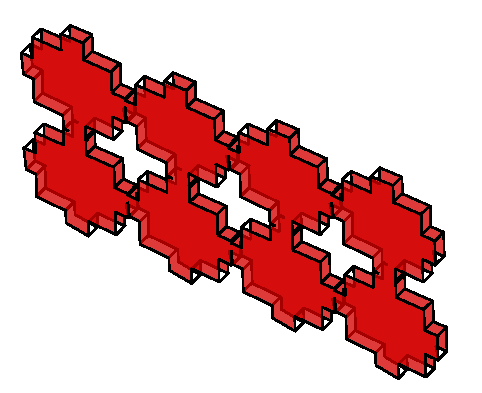
\includegraphics[width=3cm]{img/multilay_1red.pdf}
               %\caption{2gn.pdf}   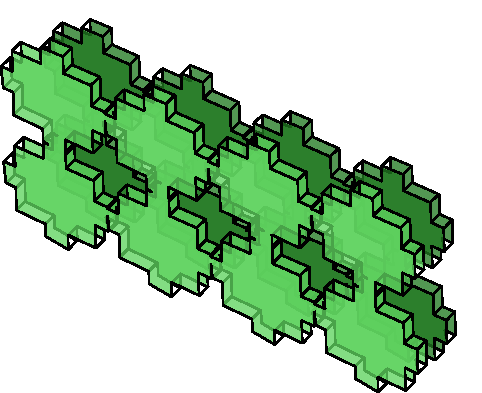
\includegraphics[width=3cm]{img/multilay_2gn.pdf}
               %\caption{3bu.pdf}   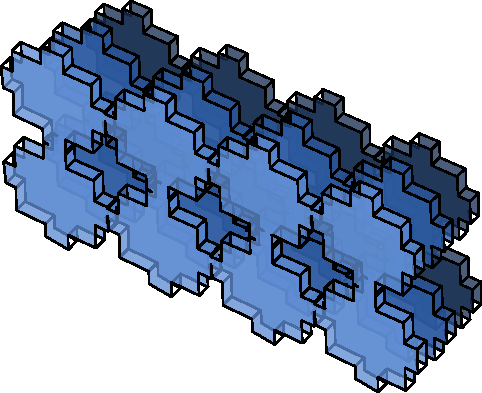
\includegraphics[width=3cm]{img/multilay_3bu.pdf}
               %\caption{3grey.pdf} 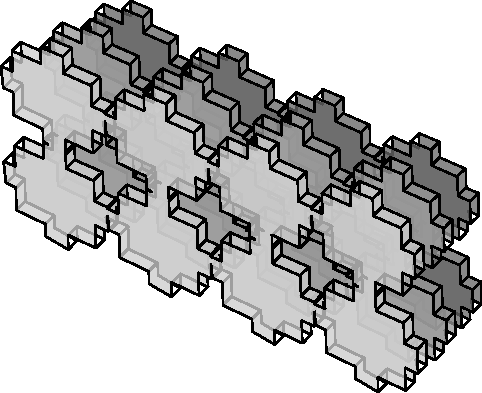
\includegraphics[width=3cm]{img/multilay_3grey.pdf}
               %\caption{4vio.pdf}  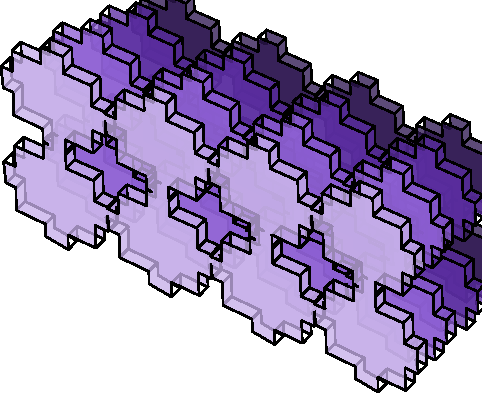
\includegraphics[width=3cm]{img/multilay_4vio.pdf} \end{figure} 

%}}}

\FloatBarrier %====================================================================================================
\section{Wire medium} \label{chap_wiremedium}
\paragraph{High-frequency behaviour}%{{{
The structure formed of a regular square lattice of conductive wires exhibits more interesting properties when the electric field is parallel to the wires, and this polarisation will be assumed in the following. The lattice of wires perpendicular to the electric field does not appreciably interact with the electromagnetic wave, until the wire thickness is of similar magnitude to their spacing; such a case is discussed in another Section \ref{section_eot}.

In the high-frequency part of the spectrum above the first photonic band, where more than a half wave fits into the unit cell, the layers of metallic rods can be approximated by thin scattering slabs from the previous section, since the high-frequency interaction of the wave can be described of photonic bands alternating with Bragg band gaps. In contrast with the dielectric PhC described above, no Fabry-Pérot resonances are observed and the scattering strength of the wire layers reduces monotonously with growing frequency.

\begin{figure}[bh] \caption{Amplitude of \textbf{(a)}  reflectance, \textbf{(b)} transmittance \textbf{(c)} effective index of refraction $\Neff$ and \textbf{(d)} effective permittivity $\eeff$ for the array of wires made of gold, depending on the wire radius $\rho_w \in \{1, 2, 4, 8, 16\}$ $\mu$m with a fixed unit cell size $a = 100$ $\mu$m and grid resolution of 1 $\mu$m. } \label{fg_Slab_fillfraction015_wireradius_scan} \centering \vspace{-3mm}
\begin{tabular}{r}
\begin{overpic}[width=0.85\textwidth]{img-meep/Wires_wireradiusscan_r.pdf} \put (-1,28) {\textbf{(a)}} \end{overpic}\vspace{-0.060\textwidth}\\ 
\begin{overpic}[width=0.85\textwidth]{img-meep/Wires_wireradiusscan_t.pdf} \put (-1,28) {\textbf{(b)}} \end{overpic}\vspace{-0.057\textwidth}\\
\begin{overpic}[width=0.86\textwidth]{img-meep/Wires_wireradiusscan_n.pdf} \put (-1,28) {\textbf{(c)}} \end{overpic}\vspace{-0.055\textwidth}\\
\begin{overpic}[width=0.86\textwidth]{img-meep/Wires_wireradiusscan_eps.pdf} \put (-1,28) {\textbf{(d)}} \end{overpic}\vspace{-0.030\textwidth}\\
\end{tabular}
\end{figure}

%}}}
\paragraph{Inductive behaviour at low-frequencies}%{{{
At low frequencies, in contrast, the interaction of the conductive wires with the electromagnetic wave becomes very strong and leads to completely different behaviour than that described above. For a frequency range from zero up to the \textit{effective plasma frequency} $f_p$, the array exhibits a band gap where $\Neff$ is pure imaginary and $k'\approx 0$. Therefore, in the low-frequency part of the spectrum, the local effective permittivity $\eeff$ is a physically meaningful quantity and follows the law typical of inductive media:
\begin{equation} \eeff(f) = 1 - \frac{f^{2}}{f_p^{2}}\label{eq_eeff_plasma}\end{equation}
Such a dependence of $\epsrl$ was already used in the Drude model in Eq. (\ref{eq_drude_eps}), and plotted in Fig. \ref{fg_Au_models}. Owing to this similarity to metals or plasma, wire arrays are denoted also as \textit{diluted metal} or \textit{artificial plasma} since 1950s \cite{merkel1973simulation, rotman1962plasma}, or as \textit{metallic delay dielectrics}, owing to the possibility to manipulate the phase and group velocities  \cite[p. 54]{brown1953artificial}.

The physical origin of $\eeff<0$ is different than in continuous media, where it is \textit{kinetic}, i.e., due to the effective mass of electrons. In contrast, the negative effective permittivity in wire arrays is the result of the \textit{self inductance} due to the magnetic field circulating around the conductor. 

Except for optical frequencies, $f_p$ does not substantially depend on the internal plasma frequency of the constituent metal, and such behaviour can be obtained even if wires are thought to be made of a perfect electric conductor (PEC).
The plasma frequency does, however, depend on the geometry described by two parameters, the wire radius $\rho_w$ and the unit cell size $a$. 

%}}}
\paragraph{Behaviour close to the effective plasma frequency}%{{{
The dependence of $f_p$ on the wire radius $\rho_w \in \{1, 2, 4, 8, 16\}$ $\upmu$m is illustrated by the spectra of reflectance, transmittance, refractive index and effective permittivity in Fig. \ref{fg_Slab_fillfraction015_wireradius_scan}. The effective plasma frequency $f_p$ can be easily determined as the point where $\eeff'(f)$ crosses zero  in the plot \ref{fg_Slab_fillfraction015_wireradius_scan}d. This coincides with the lower edge of the first photonic band in Fig. \ref{fg_Slab_fillfraction015_wireradius_scan}c. 

For the limit $f \rightarrow f_p+$, the phase velocity $c/n = c/\sqrt{\eeff(f)}$ is proportional to $(f-f_p)^{-1/2}$ and thus very high. Conversely, the group velocity $v_g \approx 2\pi \mathrm{d}f/\mathrm{d}k = \mathrm{d}f/\mathrm{d}n$ vanishes, being proportional to $(f-f_p)^{+1/2}$. The product of the phase and group velocities close to $f_p$ thus remains nearly constant $c^2$, which is a phenomenon commonly encountered also near the \textit{cut-off frequency} of metallic waveguides.

Exactly at $f=f_p$, the wire array medium can support the longitudinal oscillations of the charge, oriented parallel to the wires. They bear a close resemblance to plasmons in bulk media \cite{pendry1996extremely}.

Notice that for a single cell, the transition from negative to positive permittivity is not accompanied by any obvious spectral feature on the reflection/transmission plot. Except for the zero frequency, a layer of wires has always nonzero transmittance that increases with frequency. Independent of the wire conductivity, it is not possible to build a 100\% efficient wire polarizer.

\begin{figure}[th]
  \begin{minipage}[c]{0.69\textwidth}
\begin{overpic}[width=.98\textwidth]{img/EWire_plasmaF_spacingscan.pdf} \put (-1,60) {\textbf{(a)}} \end{overpic}\\
\begin{overpic}[width=\textwidth]{img/EWire_plasmaF_radiusscan.pdf}  \put (-1,58) {\textbf{(b)}} \end{overpic}\\
  \end{minipage}
  \begin{minipage}[c]{0.3\textwidth}
	  \caption{Comparison of numerical results and analytic models for plasma frequency $f_p$ of a wire medium.\\ \textbf{(a)} $f_p$ as a function of wire spacing. \\ \textbf{(b)} $f_p$ as a function of wire radius $\rho_w$.}\vfill \label{fg_omegap_a}
  \end{minipage}  
\end{figure} 

%}}}
\paragraph{Plasma frequency as a function of wire radius and unit cell size}%{{{
From Fig.  \ref{fg_Slab_fillfraction015_wireradius_scan}, it can be also deduced that $f_p$ is approximately proportional to the logarithm of $\rho_w$ if $\rho_w \ll a$. This is related to that a thicker wire should have slightly lower inductance per unit length (sometimes denoted as its \textit{self-inductance}). 

The effect of wire spacing $a$ is the opposite; with $a$ growing, the magnetic field has more space to circulate around the wir and $f_p$ reduces. 

Different analytic models were proposed for description of both effects. The early model by Pendry \textit{et al.} from 1996 \cite{pendry1996extremely} works well for thin wires: 
\begin{equation} f_p(\rho_w,a) \approx \sqrt{\frac{c^2}{2\pi \, a^2 \, \ln(\frac{a}{\rho_w})}}. \label{eq_fp_pendry}\end{equation}
Its refinement by Maslovski \textit{et al.} from 2003 \cite{maslovski2002wire} should be valid also for wires with relatively high fill fraction:
\begin{equation} f_p(\rho_w,a) \approx \sqrt{\frac{c^2}{2\pi \, a^2 \, \ln\left(\frac{a^2}{4\rho_w (a-\rho_w)}\right)}} \label{eq_fp_maslovski}\end{equation}

We ran two series of wire array simulations as a simple verification of both the FDTD algorithm against the mentioned analytic models. In the first series plotted in Fig. \ref{fg_omegap_a}a, we kept the wire radius constant $r = 16\,\upmu$m  and changed the wire spacing $a$ (red points). For comparison, we plot in the plasma frequency predicted by both analytic models from Eqs. (\ref{eq_fp_maslovski}, \ref{eq_fp_pendry}) as full and dotted lines, respectively. 

To test the possible error introduced by the FDTD algorithm, we ran the simulation with different resolution - results with fine $1$ $\upmu$m grid are denoted by full circles, results with coarse $4$ $\upmu$m grid with empty squares. Finally we also repeated this plot for thinner wire with $r = 8$ $\upmu$m. %%todo rewrite?

In the second series of simulations plotted in Fig.  \ref{fg_omegap_a}b, we kept the spacing $a = 100\,\upmu$m and changed the wire radius $r$. The analytic model and FDTD simulation give similar results (up to 5 \%) even for wire radii approaching roughly $a/4$. For thicker wires, the analytic model predicts higher plasma frequency than FDTD.  To conclude, the results of the model presented by Maslovski match the FDTD simulation with good accuracy for thin wires (where $r \lesssim a/5$). One possible application of the wire medium is in the construction of negative refractive index metamaterials, where a small negative real value of effective permittivity is desired.%%todo rewrite?

%}}}
%TODO \paragraph{Oblique propagation of the wave} % {{{
%ref Homogenisation of nonlocal media such as wires 
%\cite{capolino2009book}
%\cite{silveirinha2007metamaterial}
%\cite{belov2003strong}
%\cite{belov2002dispersion}
%\cite{silveirinha2005homogenization}
% nice refs  from 1950-1970: http://ece-research.unm.edu/summa/notes/SSN/note192.pdf

%}}}

\FloatBarrier %====================================================================================================
\section{Cut wires} \label{section_cutwires}
\paragraph{Individual resonances}%{{{
The low-frequency behaviour of the wire array is determined by the distributed inductance of the wires, which introduces negative effective permittivity up to the plasma frequency $f_p$. When the wires are cut in each unit cell, a three-dimensional periodic lattice of antennas is formed. Its important parameters are not only the inductance along each antenna, but also the capacitance across the gap between wires. In an analogy with a series LC (coil-capacitor) circuit, such antennas exhibit \textit{individual resonances} at some nonzero resonant frequency $0<f_r<f_p$. 

These resonances couple to the electromagnetic field by means of their electric dipole, and are thus denoted shortly as \textit{electric resonances}. This does not mean that no magnetic field is involved; in fact, the energy is exchanged between the resonant electric and magnetic fields each quarter-period. The situation partially changes with decreasing size of the particles. At optical frequencies, the energy is exchanged between the electric field and the kinetic energy of the electrons, while the magnetic field circulating around the metallic particle plays a minor role only. Such regime is known as \textit{plasmonic resonances} and was described by Mie in 1908 \cite{mie1908beitrage}.

The spectra for the cut-wire structure are depicted in Fig. \ref{fg_CutWires_wireradius1u_cutwidth_comparison} for different cut distances $d_c$. Starting with the thinnest wire of $\rho_w = 2$ $\upmu$m (red curve), we can identify the individual resonance as the point close to  1200 GHz where even a single layer of unit cells reflects full wave amplitude and the transmittance drops to zero. Towards higher or lower frequencies from the resonance, the transmittance is relatively high.

%% TODO check if the spatial dispersion would be visible in the CDH plots
%% ...even here, with particles infinitesimally thin along the wave-vector, the spatial dispersion may be significant; arguably it was observed in 1970s by Merkel \cite{merkel1973simulation}, who remarks that
%% "It is interesting that the more exact expressions for the dielectric constant of the artificial dielectric, which considered both the effect of the capacitive dipole impedance and the dipole-dipole interaction, did not model the behavior of a Lorentzian plasma as well as the original simplified approach"
%% TODO note about plasmonic particles 
%}}}
\begin{figure}[h!] \caption{Amplitude of \textbf{(a)} reflectance, \textbf{(b)} transmittance, \textbf{(c)} effective index of refraction $\Neff = \Neff' + \ii \Neff''$ for the array of cut wires of radius $r_w = 1$ $\upmu$m made of gold, depending on cut distance $r_w\in \{2, 4, 8, 16, 32, 64\}$ $\upmu$m. The unit cell is cubic and its size is $a=100$ $\upmu$m.\\%{{{
In plot  \textbf{(d)}, the effective permittivity is illustrated for the thinnest cut distance $d_c = 2$ $\upmu$m. Although retrieved for the entire spectrum, the local effective parameters have physical meaning only when the wavelength is much larger than $a$, i.e. roughly from 0 to 500 GHz and from 1220 to 1280 GHz.} \label{fg_CutWires_wireradius1u_cutwidth_comparison} \centering \vspace{-3mm}
\begin{tabular}{r}
\begin{overpic}[width=0.85\textwidth]{img-meep/CutWires_wireradius1u_cutwidth_comparison_r.pdf} \put (-1,28) {\textbf{(a)}} \end{overpic}\vspace{-0.059\textwidth}\\
\begin{overpic}[width=0.85\textwidth]{img-meep/CutWires_wireradius1u_cutwidth_comparison_t.pdf} \put (-1,28) {\textbf{(b)}} \end{overpic}\vspace{-0.056\textwidth}\\
\begin{overpic}[width=0.86\textwidth]{img-meep/CutWires_wireradius1u_cutwidth_comparison_n.pdf}\put (-1,28) {\textbf{(c)}} \end{overpic}\vspace{-0.056\textwidth}\\
\begin{overpic}[width=0.85\textwidth]{img-meep/CutWires_wireradius1u_cutwidth_comparison_eps_r2.pdf} \put (-1,28) {\textbf{(d)}} \end{overpic}\vspace{-0.030\textwidth}\\
%\begin{overpic}[width=0.85\textwidth]{img-meep/CutWires_wireradius1u_cutwidth_comparison_ni.pdf}\put (-1,28) {\textbf{(d)}} \end{overpic}\vspace{-9.5mm}\\ \begin{overpic}[width=0.85\textwidth]{img-meep/CutWires_wireradius1u_cutwidth_comparison_eps_r2.pdf}\put (-1,28) {\textbf{(d)}} \end{overpic}\vspace{-0.030\textwidth}\\
\end{tabular}
\end{figure}
%}}}
\paragraph{Dispersion near an individual resonance}%{{{
Each individual resonance in a periodic structure forms a characteristic shape in the spectrum of effective index of refraction $\Neff(f)$. The following description will therefore be applicable to individual resonances in other resonant structures, as well. 

\begin{enumerate}
\item{At frequencies under the resonance, the electric dipole of the antenna oscillates in phase with the driving field and the resonance contributes the effective index of refraction $\Neff'(f)$. 
The spectrum of a periodic structure with an individual resonance differs from the spectrum of a homogeneous medium that was already described at the Lorentzian resonance curve in Fig. \ref{fg_oscillator_spectrum}b.
At some frequency $f \lesssim f_r$ below the resonance, the index of refraction $\Neff'(f)$ becomes high enough to join the closest Brillouin zone boundary which was above it. From this point up to the resonance frequency $f_r$, $\Neff(f)$ has nonzero imaginary part, and the medium exhibits a band gap.
} 
\item{Exactly at the resonance frequency, the interaction of the dipole with the field changes its sign, since above the resonance, the dipole starts to be oriented opposite to the driving field. 
The real part of the refractive index $\Neff'(f)$ ceases to follow one Brillouin zone and transitions to another Brillouin zone below it. In local media, individual resonances appears to be the only occasions for $\Neff'(f)$ to transition downwards.

The imaginary part of the refractive index, $\Neff''(f)$, is required by the Kramers-Kronig relations to exhibit a sharp peak at the resonance frequency, which is superposed over the broader background stemming from the band gap (see Fig. \ref{fg_CutWires_wireradius1u_cutwidth_comparison}c). 

The spectral width of the transition and peak is inversely proportional to the quality of the resonance. Whenever the structure is built from realistic materials with nonzero losses and its spatial dispersion can be neglected, $\Neff(f)$ is a continuous complex function.
} 
\item{The band gap continues up to some frequency $f > f_r$, where another photonic band begins between the same pair of Brillouin zones.  
} 
\end{enumerate}

The most important observation is that the resonance curve of $\Neff(f)$ in periodic structures is constrained between the closest two Brillouin zone boundaries, which can be understood as the "floor" and "ceiling" for the dispersion curve. Apparently a single individual resonance can not shift the transmittance phase by more than $\pi$ per each layer of unit cells. It can therefore introduce a band of imaginary $\Neff$, but for $\Neff$ to reach negative values, two resonances must be combined.

The impact of the individual resonances on the effective parameters $\eeff(f)$ and $\meff(f)$ will be discussed in the later section focused on the dielectric resonators. % TODO verify that I have done this

%}}}
\paragraph{Effects of the cut distance $d_c$}%{{{
An increase of the cut distance $d_c$ clearly increases the resonance frequency $f_c$. The reason is twofold: for a cut width small relative to the unit cell size, $d_c\ll a$, it is mostly due to reduced capacitive coupling between the cut wires; for cut width comparable or greater than the unit cell size, $d_c \gtrsim a$, reduction of the cut-wire inductance is more important.

Both the individual and Bragg-type resonances can be identified in the plot for different $d_c$ in Fig. \ref{fg_CutWires_wireradius1u_cutwidth_comparison}c. When $d_c \sim 16$  $\upmu$m, the individual resonance shifts above 1.5 THz and exchanges its order with the Bragg band gap. 
For $d_c \gtrsim 32$  $\upmu$m on, the individual resonances are similar to those for a $d_c\sim 2$ $\upmu$m, but are shifted by one Brillouin zone up.

%}}}
\begin{figure}[h!] \caption{Amplitude of \textbf{(a)} reflectance, \textbf{(b)} transmittance and \textbf{(c)} effective index of refraction $\Neff = \Neff' + \ii \Neff''$ for a metamaterial made of cut wires. Cut distance $d_c = 2$ $\upmu$m, unit cell size $a=100$ $\upmu$m.} \label{fg_CutWires_wirecut2um_wireradiusscan} \centering \vspace{-3mm} %{{{
\begin{tabular}{r}
\begin{overpic}[width=0.85\textwidth]{img-meep/CutWires_wirecut2um_wireradiusscan_r.pdf} \put (-1,28) {\textbf{(a)}} \end{overpic}\vspace{-0.060\textwidth}\\
\begin{overpic}[width=0.85\textwidth]{img-meep/CutWires_wirecut2um_wireradiusscan_t.pdf} \put (-1,28) {\textbf{(b)}} \end{overpic}\vspace{-0.060\textwidth}\\
\begin{overpic}[width=0.85\textwidth]{img-meep/CutWires_wirecut2um_wireradiusscan_n.pdf}\put (-1,28) {\textbf{(c)}} \end{overpic}\vspace{-0.030\textwidth}\\
	% TODO GIT ADD - update pic 
\end{tabular}
\end{figure}
%}}}
\paragraph{Effects of the wire radius $\rho_w$}%{{{
The dependence of the resonance frequency $f_c$ on the wire radius, Fig. \ref{fg_CutWires_wirecut2um_wireradiusscan}, is somewhat more complicated: For thin enough wires in the $a=100$ $\upmu$m unit cell, the resonance frequency decreases with growing $\rho_w$, since the inter-wire capacity increases. 
For high enough $\rho_w$ an opposite mechanism prevails; $f_c(\rho_w)$ then starts growing as a result of reduction of the wire inductance.

While the change of the cut-wire radius $\rho_w$ relatively weakly reflects in the resonance frequency, its major impact is in the \textit{strength} of the individual resonance. Thick wires lead to stronger reflection out of resonances, which also translates into a wider band gap in Fig. \ref{fg_CutWires_wirecut2um_wireradiusscan}c.


% TODO
% \paragraph{Experimental measurement of cut wire spectra}
% \todo{origin of samples, semi-conductive si substrate, compute spectra, plot graphs and compare with experiment}
% \begin{figure}[ht] \caption{The sample of cut wires (pale yellow) on silicon (cyan) substrate. \textbf{(a)} Natural-colour photograph from an optical microscope,  \textbf{(b)} Geometry of the wires in micrometers. They were measured to be $6.5$ $\mu$m wide and $30$ $\mu$m long. The periodicity of cut-wires was $30\times 50$ $\mu$m.  } \label{fg_sieving2} \centering 
% 	\begin{overpic}[height=.40\textwidth]{img/bousek_splitwires_microphoto.pdf}  \put(0,78) {\textbf{(a)}} \end{overpic}
% 	\begin{overpic}[height=.40\textwidth]{img/bousek_splitwires_drawing.pdf}  \put(0,95) {\textbf{(b)}} \end{overpic}
% \end{figure}
%}}}

%     \FloatBarrier %====================================================================================================
%     \section{Electric resonators} \label{section_esrr} % references to -> % note about plasmonic particles 
%     \paragraph{Comparison of spectra to the cut wires}%{{{
%     From Figs. \ref{fg_CutWires_wirecut2um_wireradiusscan} and \ref{fg_CutWires_wireradius1u_cutwidth_comparison} it follows that for any practically attainable geometry, the frequency of the first individual resonance in cut-wire arrays is always relatively close to the first Bragg band gap. 
%     
%     A viable way to shift the resonance frequency much lower, without changing the unit cell size nor resorting to submicrometre cut distances, is to replace straight wire antennas by \textit{electric split-ring resonators}, % TODO cite 
%     depicted in Fig. \ref{fg_eSRR}.
%}}}

\FloatBarrier %====================================================================================================
\section{Split-ring resonator} \label{section_srr} % references to -> 
\paragraph{Resonances with magnetic dipole moment}%{{{
The fundamental resonance in a cut wire has the electric dipole moment only. The resonant magnetic field circulates around the wire and due to its rotational symmetry along the $x$-axis, the magnetic dipole moment is zero. Other structures can support resonances of lower symmetry with regards to the $x$-axis, thus having a magnetic dipole moment.

One of the simplest examples is formed by bending the wire into a "C"-shaped \textit{split-ring resonator} (SRR). To reduce the resonant frequency, capacitor pads can be added to the cut, as shown in Fig. \ref{fg_SRR_types}a. The first resonance in its spectrum has a dominant magnetic dipole moment, and will be denoted simply as a \textit{magnetic resonance}. The electric current flows through the wire along a circular path, while the magnetic field has a toroidal shape around the wire.   

The very concept of SRR is at least as old as the Hertz's experiments with the spark-gap transmitter from 1880s.
As described in the historical review of Ref. \cite[pp. 120--126]{solymar2009waves}, first SRR arrays were built in early 1980s with the aim to build an effective medium with highly lossy complex permeability; a decade later asymmetric SRRs were used to achieve strong bianisotropy. Many publications cite Refs. \cite{pendry1999magnetism,pendry2000negative} from Pentdry et al. as the first application of SRR array for achieving negative effective permeability and index of refraction, respectively. Since then, the number of SRR-related publications has grown rapidly. 
\label{negn_srr}

\begin{figure}[h] \caption{Variants of the split-ring resonators, viewed from the side perpendicular to the magnetic field: \textbf{(a)} classical SRR, \textbf{(b)} symmetric SRR with two splits, \textbf{(c)} one of the designs of an electric SRRs having a central bar, \textbf{(d)} a similar structure where the central bar was split by a capacitor with pad radius $\rho_c$, allowing to tune the electric resonance} \label{fg_SRR_types} \centering 
\begin{overpic}[height=0.25\textwidth]{img/drawing_SRRpad.pdf}\put (1,80) {\textbf{(a)}}\end{overpic}\qquad
\begin{overpic}[height=0.25\textwidth]{img/drawing_sSRRpad.pdf}\put (1,80) {\textbf{(b)}}
		\put(110,30){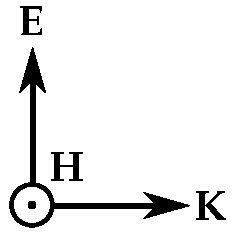
\includegraphics[width=.12\textwidth]{img/tripletEHK.pdf}}
\end{overpic}\qquad
\end{figure}

%}}}
\paragraph{Symmetry of the split-ring}%{{{
The orientation of the splitting in the SRR determines the possible coupling between its electric and magnetic dipoles. In particular, when the splitting is on the front or rear side of the ring relative to the  direction of wave propagation, the predominantly magnetic resonance creates also a weak electric dipole, leading to the optical activity.

Reduced symmetry with regards to the wave propagation may even break the homogenisation based on scattering parameters retrieval, as this procedure assumes that the structure is symmetric, i.e., its reflectance is equal from both sides. Asymmetric structures therefore have properties that can not be matched by any (reciprocal) homogeneous medium. 

The symmetry is restored again by considering a \textit{symmetric split ring resonator} (sSRR), depicted in Fig. \ref{fg_SRR_types}b, which has two splittings at opposing position on the ring. 
% A. Andryieuski, C. Menzel, C. Rockstuhl, R. Malureanu, and A.V. Lavrinenko, The split cube in a cage: %bulk negative-index material for infrared applications, Journal of Optics A: Pure and Applied Optics,
%vol. 11, p. 114010, 2009.
This is documented by the results in \ref{fg_SRR_principles}. The SRR with a single splitting is represented by red lines; while its magnitude of reflectance and transmittance in Fig. \ref{fg_SRR_principles}a,b appear similar to these of a cut wire, the computation of the refractive index yields a spectrum (Fig. \ref{fg_SRR_principles}c) which has no reasonable interpretation near the resonance at 500 GHz and above it. 

The symmetric resonator is represented by green curves. In Fig. \ref{fg_SRR_principles}c, the refractive index follows a resonance pattern that was already described on the example of the cut wires: the curve grows up to the upper Brillouin zone boundary, follows it for a span of frequencies, drops to the Brillouin zone boundary below, follows it again and then a next band starts. 

At higher frequencies, outside the range of Fig. \ref{fg_SRR_principles}, the SRR exhibits also the electric resonance where the current flows symmetrically along both its arms. It is assumed that any structure should support infinite number of resonances, of which only the lowest few are usually of any interest.
%}}}
\paragraph{Antiresonances in local effective parameters}%{{{
In the case of symmetric split-ring resonators, the first resonance possesses only the magnetic dipole moment, as follows from the symmetry of the resonant fields. This fact reflects in a strong resonant behaviour of the permeability $\meff(f)$ (green curve in Fig. \ref{fg_SRR_principles}e, between 600 and 700 GHz). 

The permittivity spectrum $\eeff(f)$ is, however, also affected by the magnetic dipole resonance  (Fig. \ref{fg_SRR_principles}d). The impact of the magnetic resonance on $\eeff(f)$ is several times weaker than on $\meff(f)$, and more importantly, it has an opposite sign: The real part of $\eeff'(f)$ is reduced at frequencies below the resonance, and increased above it. Simultaneously, the sign of the imaginary part $\eeff''(f)$ would imply amplification of the electric field oscillating around 650 GHz, which is impossible in a structure composed of lossy materials only. This feature in the spectrum is sometimes described as an \textit{antiresonance} and has incited much discussion in the literature \cite{koschny2003resonant, wallen2011anti}. 
%}}}
\paragraph{Physical relevance of effective parameters in their local approximation}%{{{
We believe that the influence of a magnetic resonance on $\eeff(f)$, or conversely, of an electric resonance of $\meff(f)$, is a mere artifact of approximating a strongly nonlocal structure with a concept of local effective parameters. It can be shown antiresonances become stronger at higher frequencies, as the wavelength $2\pi/K$ becomes similar to the unit cell size $a$. 
In Ref. \cite{wallen2011anti}, it is argued that % against this interpretation with
\begin{displayquote}
\textit{the periodicity cannot \ldots be the only explanation since qualitatively similar antiresonances have been reported using the measured data for a disordered high permittivity composite.}
\end{displayquote}
The true origin of antiresonances and other deviations of $\eeff(f)$ and $\meff(f)$ from the Lorentzian resonance curve can however be attributed to the presence of photonic band gaps and nonlocal response of the structure. These effects are, to some extent, maintained also under randomizing the unit cell positions \cite{peng2007},   
thus there is probably no need to seek for another explanation. %%TODO rewiew, rewrite?
% \cite{alu2010} "Restoring the physical meaning of MM constitutive parameters"

%An elaborate comparison of resonant metallic structures, with clear effect of adding the wire to the transmission spectra, can be found e.g. in Ref. \cite{koschny2004effective}.

%Ref. \cite{li2009determination} contains typical complex-valued spectra of $\eeff$ and $\meff$ for a SRR and SRR-Wire
% different orientations - some leading to chirality i.e. linear dependence of f(K)
% when not failing due to chirality, s-param yields beautifully similar results to our simulations!
% "CMM = Composite MetaMaterial"
%}}}
\paragraph{Comparison of the s-parameters method and CDH}%{{{
With local effective parameters $\eeff(f)$ and $\meff(f)$ appearing to lose their physical meaning in a frequency range near a resonance, a question remains to what extent the dispersion curves, or equivalently, the spectrum of effective index of refraction $\Neff(f)$ is applicable. While the Bloch theorem in Eq. (\ref{eq_bloch}) suggests that the dispersion curves for the Bloch wavevector $\KK$ can be determined for any periodic structure, the s-parameter method might return invalid values.

Dispersion curves obtained by the s-parameters method and by the current-driven homogenisation (CDH) are compared in Fig. \ref{fg_cdh5}. Although these methods are fundamentally different, their results overlap, and thus one can assume that the array of symmetric split-ring resonators can be treated as homogeneous with well-defined index of refraction $\Neff(f)$ for the Bloch wave over the whole spectrum. Its local effective parameters $\eeff(f)$ and $\meff(f)$, however, seem to have no useful physical interpretation near the resonances, where the Bloch wavelength is similar to the unit cell size. They remain useful farther from the resonance, though. % todo perhaps add some particular frequency ranges from the Fig.

%}}}
\paragraph{Variants of split-ring resonators}%{{{
\begin{figure}[t] \caption{Other variants of split-ring resonators: \textbf{(a)} double SRR, \textbf{(b)} symmetric version thereof, \textbf{(c)} double SRR with cross-connection between the inner and outer rings, \textbf{(d)} illustration of a square variant of the double SRR, \textbf{(e)} the "omega" structure aimed to introduce $\Neff'<0$, \textbf{(f)} the cut-wire pair} \label{fg_SRRothers} \centering 
\begin{overpic}[height=0.22\textwidth]{img/drawing_dSRRpad.pdf}    \put (1,81) {\textbf{(a)}}\end{overpic}\quad
\begin{overpic}[height=0.22\textwidth]{img/drawing_dsSRRpad.pdf}   \put (1,81) {\textbf{(b)}}\end{overpic}\quad
\begin{overpic}[height=0.22\textwidth]{img/drawing_dSRRcrossed.pdf}\put (1,81) {\textbf{(c)}}\end{overpic}\\
\begin{overpic}[height=0.22\textwidth]{img/drawing_dSRRsquare.pdf} \put (-7,81) {\textbf{(d)}}\end{overpic}\quad
\begin{overpic}[height=0.22\textwidth]{img/drawing_SRRomega.pdf} \put (-6,81) {\textbf{(e)}}\end{overpic}\quad
\begin{overpic}[height=0.22\textwidth]{img/drawing_strippair.pdf} \put (1,81) {\textbf{(f)}}
		\put(100,30){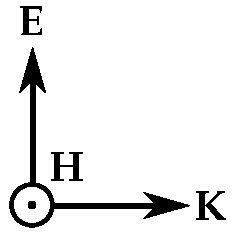
\includegraphics[width=.12\textwidth]{img/tripletEHK.pdf}}
\end{overpic}\quad
\end{figure}
Diverse metamaterial designs based on the SRR principle were developed.
Many SRR designs involve a smaller ring nested inside the original one, as shown in Fig. \ref{fg_SRRothers}a,b in the asymmetric and symmetric variants. The long narrow gap between the inner and outer split ring enhances their capacitive coupling. This way, the frequency of the magnetic resonance can be reduced without increase of the overall SRR dimensions. Such designs usually do not need capacitor pads, and can be made by etching or microlitography. 

A modification of this \textit{double split-ring} design includes cross-connection between the inner and outer conductors as in Fig. \ref{fg_SRRothers}c; this version also breaks mirror symmetry. 

The square "ring" resonator (Fig. \ref{fg_SRRothers}d) is also widely used, without any substantial difference from the round SRR.

The \textit{omega structure} was designed to emulate the operation of a SRR and a wire simultaneously, by interconnecting the ends of a SRR along the $x$-axis (Fig. \ref{fg_SRRothers}e).

All SRR structures in Fig. \ref{fg_SRRothers} can be made flat in the plane perpendicular to the magnetic field, which facilitates their fabrication. At terahertz and higher frequencies, using a thin metal film should not be much detrimental to the SRR conductivity, since the skin depth caused by eddy currents is often submicroscopic \cite{gibbons2010scalable}.

On the contrary, a similar way of operation is achieved by structures infinite in the direction of the magnetic field. This allows to fabricate magnetic resonators by rolling stripes of a semi-metallised plastic foil, producing a \textit{swiss-roll} metamaterial \cite{gibbons2010scalable}, or by partially sputter-coating a polymer fibre by metal \cite{wang2011fiber}. Such structures however seem to exhibit relatively high losses when applied above the microwave range.

Metallic \textit{cut-wire pair}, or also \textit{strip pair}, metamaterial depicted in Fig. \ref{fg_SRRothers}f, was designed for operation in the infrared or optical range. It can be understood as a split-ring resonator flattened along the direction of the wave vector. The geometry is tuned so that the electric and magnetic resonances overlap.	

%}}}
\paragraph{SRR in a wire array} %{{{
The analysis of the wire array has shown that at low frequencies, its effective permittivity is physically valid and has a negative value. Likewise, the symmetric SRR has a region in the spectrum above its magnetic resonance where its effective permeability is negative, too.

A synthesis of these two structures yields a region of negative index of refraction, probably the first \cite{pendry2000negative} and most prominent metamaterial design to achieve this. The effect of combining structures that interact exclusively with magnetic and electric field is discussed in Ref. \cite{koschny2004effective} in more detail.

The resulting effective parameters are represented by the blue line in Fig. \ref{fg_SRR_principles}. Its spectrum of the effective index of refraction resembles that of the wire array up to 630 GHz, where it drops by one Brillouin zone down at the resonant frequency.
As a general rule observed in all correctly retrieved spectra, a single individual resonance always causes $\Neff'(f)$ to drop from one Brillouin zone boundary to another. 

Notice that the magnetic resonance causes a drop in $\Neff'(f)$ even without the wire array (green curve in Fig. \ref{fg_SRR_principles}c), but in such a case it happens between the first Brillouin zone boundary and zero. Without wires, $\Neff'$ does not reach negative values.

By contrast, a magnetic resonance in the combined SRR-wire structure introduces a narrow region, still within the photonic band gap, where 
\begin{equation} \Neff(f) = -\frac{c}{2 a f}, \label{eq_BZN2}\end{equation}
with $a$ being the unit cell size.	

The photonic band spanning from 635 to 670 GHz thus has $\Neff'<0$, but only when $\Neff'$ comes closer to zero, roughly from 650 to 670 GHz, also the effective permittivity and permeability can be attributed with physical meaning. They are correctly retrieved as both negative, as can be indeed seen from in Figs. \ref{fg_SRR_principles}d,e (blue lines).

%}}}
\paragraph{Fano resonance} %{{{
The spectrum of reflectance magnitude $|r(f)|$ for the sSRR-wire structure (blue line in Fig. \ref{fg_SRR_principles}a) has a relatively complex shape -- starting from a high reflectance introduced by the wire array, it grows below the magnetic resonance, then it drops to zero around 660 GHz, and it grows until its local maximum on 750 GHz is reached.

It differs significantly from the arguably simpler spectrum of the cut wires (Figs. \ref{fg_CutWires_wireradius1u_cutwidth_comparison}a and \ref{fg_CutWires_wirecut2um_wireradiusscan}a), where the resonance was accompanied by a single peak in reflectance. Since the structures have negligible lossess, complementary observations can be made with the transmission spectrum.

The reason is in that with the sSRR-wire structure, $|r(f)|$ is a linear superposition of the wave scattered by the interaction of the structure with the electric field, which has relatively large amplitude $r_{1}(f)$ over broad spectral range, and another wave $r_{2}(f)$ scattered by the magnetic dipole which is prominent only close to the magnetic resonance, between 550 and 750 GHz.

Both scattered components, $r_1(f)$ and $r_2(f)$, are complex functions. The phase of a wave scattered by a resonant element differs almost by $\pi$ for $f$ below and above the resonance. The impact on the plot of the overall reflectance is in a change from a constructive to destructive interference between the two components. 

Such typical spectral features, observed whenever a narrower resonance overlaps with another broader one, are known as \textit{Fano resonances}, and can be found on most following plots of $|r(f)|$ or $|t(f)|$. On the contrary, when the Fano lineshape is missing in the spectrum of a structure that obviously possesses a magnetic dipole, it suggests the homogenization would have failed (see, e.g., the spectra of the asymmetric SRR in \ref{fg_SRR_principles}).  

%}}}
\begin{figure}[t] \caption{Split-ring resonator: %{{{
		amplitude of \textbf{(a)} reflectance, \textbf{(b)} transmittance, \textbf{(c)} effective index of refraction,  \textbf{(d)} effective permittivity $\eeff$ and \textbf{(e)} effective permeability $\meff$  .   %% todo check params comment=sSRR with wire_resolution=2.000e-06_capacitorr=1.000e-05_splitting=4.000e-06_wirethick=4.000e-06_splitting2=4.000e-06_radius=3.000e-05_simtime=2.000e-10
Outer ring radius $\rho = 30$ $\mu$m, conductor cross-section $\Delta\rho = 6$ $\mu$m, unit cell size $a=100$ $\mu$m. \\
Comparison of the more familiar standard SRR (split width $d=4$ $\mu$m) with its symmetric variant sSRR (double split width $d=2$ $\mu$m) and the same sSRR with wire grid added. The dispersion curves nor effective parameters for the asymmetric SRR could not be determined by the scattering parameters method. } \label{fg_SRR_principles} \centering \vspace{-3mm} 
\begin{tabular}{r}
\begin{overpic}[width=0.85\textwidth]{img-meep/SRR_principles_r.pdf} \put (-1,28) {\textbf{(a)}} \end{overpic}\vspace{-0.060\textwidth}\\
\begin{overpic}[width=0.85\textwidth]{img-meep/SRR_principles_t.pdf} \put (-1,28) {\textbf{(b)}} \end{overpic}\vspace{-0.060\textwidth}\\
\begin{overpic}[width=0.85\textwidth]{img-meep/SRR_principles_n.pdf}\put (-1,28) {\textbf{(c)}} \end{overpic}\vspace{-0.060\textwidth}\\
\begin{overpic}[width=0.85\textwidth]{img-meep/SRR_principles_eps.pdf}\put (-1,28) {\textbf{(d)}} \end{overpic}\vspace{-0.060\textwidth}\\
\begin{overpic}[width=0.85\textwidth]{img-meep/SRR_principles_mu.pdf}\put (-1,28) {\textbf{(e)}} \end{overpic}\vspace{-0.030\textwidth}\\
\end{tabular}
\end{figure}
\begin{figure}[h] \caption{Current-driven homogenization results, shown as bubbles,  indicating the dispersion curves 
	for \textbf{(a)} a symmetric split-ring resonator and \textbf{(b)} the same with a wire mesh. The results of the scattering-parameters method are overlayed as green lines; these show the same data as the green and blue solid lines from Fig. \ref{fg_SRR_principles}c. In the right panel, the negative-index range of frequencies between 630 and 670 GHz was mirrored against the $K=0$ vertical axis and plotted by a dashed green line.} \label{fg_cdh5} \centering  % todo add params SRRArray_comment=symmetric SRR_simtime=2.000e-10_wirethick=0.000e+00_splitting2=1.600e-05_radius=3.000e-05_model=SRRArray.pdf
	% TODO recalculate and update
	\vspace{.1\textwidth}
	\begin{overpic}[width=.48\textwidth]{img-cdh/cdh_sSRR.pdf}  
	\put(1,96) {\textbf{(a)}} 
	\put(18,100){
\includegraphics[width=.1\textwidth]{img/drawing_sSRRpad.pdf}}
	\put(31,105){sSRR}
	\end{overpic}
	\begin{overpic}[width=.48\textwidth]{img-cdh/cdh_sSRR_wire.pdf}  
	\put(16,100){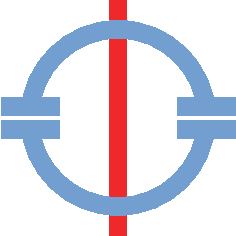
\includegraphics[width=.1\textwidth]{img/drawing_sSRRpad_wire.pdf}}
	\put(29,105){sSRR + wire}
	\put(1,96) {\textbf{(b)}} 
	\end{overpic}
\end{figure}

% todo possibly recalculate CDH for the SRR as in \ref{fg_SRR_principles}
%\begin{figure}[h] \caption{Current-driven homogenization results for the split-ring resonator \textbf{(a)} without the wire mesh and \textbf{(b)} with the wire mesh. 
	%} \label{fg_cdh4} \centering 
	%\begin{overpic}[width=.48\textwidth]{img-cdh/cdh_SRR.pdf}  \put(1,96) {\textbf{(a)}} \end{overpic}
	%\begin{overpic}[width=.48\textwidth]{img-cdh/cdh_SRRWire.pdf}  \put(1,96) {\textbf{(b)}} \end{overpic}
%\end{figure}
%}}}


\FloatBarrier %====================================================================================================
\section{Combined electric and magnetic resonator} \label{section_srr} % references to -> 
\paragraph{Effect of the central bar in SRR}%{{{
The fundamental resonance of a split-ring resonator (SRR) is the magnetic one, where the current circulates around its circumference. When one adds a central bar parallel to the electric field and the $x$-axis, as in Fig. \ref{fg_SRR_elmag}a, the frequency of the magnetic resonance does not change significantly. The reason comes from the symmetry thereof, which stipulates that that zero net current flows through the central bar. 

However, a new electric resonance (Fig. \ref{fg_emcSRR_resonances}b) is introduced by adding the bar, characteristic by that the current conducted by the central bar is antiparallel to the current conducted by both SRR arms. The corresponding frequency is lower compared to the original parallel electric resonance (Fig. \ref{fg_emcSRR_resonances}c), and similar to the frequency of the magnetic resonance (Fig. \ref{fg_emcSRR_resonances}a).  
\begin{figure}[h] \caption{\textbf{(a)} A modification of a split-ring resonator with a central bar, \textbf{(b)} a similar structure where the central bar was split by a capacitor with pad radius $\rho_c$, allowing to tune the antiparallel electric resonance} \label{fg_SRR_elmag} \centering 
\begin{overpic}[height=0.25\textwidth]{img/drawing_eSRRpad.pdf}\put (1,80) {\textbf{(a)}}\end{overpic}\quad\quad\quad
\begin{overpic}[height=0.25\textwidth]{img/drawing_emcSRRpad_sizes.pdf}\put (1,80) {\textbf{(b)}}\end{overpic}
\end{figure}
\begin{figure}[b] \caption{Three low-frequency resonances in the combined SRR: \textbf{(a)} magnetic resonance, \textbf{(b)} antiparallel electric resonance, \textbf{(c)} parallel electric resonance.\\ The actual order of the first two resonances in the spectrum is determined by the inner capacitor radius $\rho_c$ or other parameters of the structure.} \label{fg_emcSRR_resonances} \centering 
\begin{overpic}[height=0.22\textwidth]{img/drawing_emcSRRpad_resM.pdf}\put (1,81) {\textbf{(a)}}\end{overpic}\quad
\begin{overpic}[height=0.22\textwidth]{img/drawing_emcSRRpad_resE2.pdf}\put (1,81) {\textbf{(b)}}\end{overpic}\quad
\begin{overpic}[height=0.22\textwidth]{img/drawing_emcSRRpad_resE2b.pdf}\put (5,54) {\textbf{(c)}}
		\put(100,10){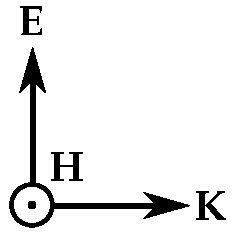
\includegraphics[width=.1\textwidth]{img/tripletEHK.pdf}}
\end{overpic}\qquad\quad
\end{figure}

%}}}
\paragraph{Tuning the frequency of the antiparallel electric resonance}%{{{
The spectra of the cut wires (Fig. \ref{fg_CutWires_wireradius1u_cutwidth_comparison}) suggest that each electric resonance, if not preceded by a Bragg band gap or excessively lossy, introduces a region in spectrum where the local effective permittivity has a physically meaningful and negative value. Under the same condition in Fig. \ref{fg_SRR_principles}, the magnetic resonance introduces a region of $\meff(f) < 0$.
\begin{figure}[t] \caption{Combined electric-magnetic resonator: amplitude of \textbf{(a)} reflectance, \textbf{(b)} transmittance and \textbf{(c)} effective index of refraction $\Neff = \Neff' + \ii \Neff''$.  
% todo check the structure parameters
%Outer ring radius $\rho = 30$ $\mu$m, conductor cross-section $\Delta\rho = 6$ $\mu$m, unit cell size $a=100$ $\mu$m. \\
%Comparison of the more familiar standard SRR (split width $d=4$ $\mu$m) with a symmetric SRR (double split width $d=2$ $\mu$m) and the same symmetric SRR with wire grid added.  The effective parameters for the asymmetric SRR could not be determined by the scattering parameters method.  %TODO params and comment 
The frequency of the electric resonance is influenced by the radius $\rho_c$ of the capacitor on the central spoke.
} \label{fg_emSRR_icr} \centering \vspace{-3mm} 
\begin{tabular}{r}
\begin{overpic}[width=0.85\textwidth]{img-meep/emSRR_inner_capacitor_radius_scan_r.pdf} \put (-1,28) {\textbf{(a)}} \end{overpic}\vspace{-0.060\textwidth}\\
\begin{overpic}[width=0.85\textwidth]{img-meep/emSRR_inner_capacitor_radius_scan_t.pdf} \put (-1,28) {\textbf{(b)}} \end{overpic}\vspace{-0.060\textwidth}\\
\begin{overpic}[width=0.85\textwidth]{img-meep/emSRR_inner_capacitor_radius_scan_n.pdf} \put (-1,28) {\textbf{(c)}} \end{overpic}\vspace{-0.030\textwidth}\\
\end{tabular}
\end{figure}

By optimizing the structure geometry, the resonances can be tuned against each other so that the regions of $\eeff(f) < 0$ and $\meff(f) < 0$ overlap. This is the conventional approach to design a metamaterial with a negative index of refraction; applying it to the electro-magnetic resonator leads to an array of independent, nonconnected elements, which may be an advantage over embedding SRRs in a wire array. One of the means of tuning the antiparallel electric resonance frequency is to divide the central bar by an \textit{inner} capacitor as shown in Fig. \ref{fg_SRR_elmag}b. 

For the inner capacitor being relatively small, with radius $\rho_c = 6$ $\upmu$m, the electric resonance is located around 1150 GHz, and it shifts down to 940 GHz when $\rho_c$ is increased to 8 $\upmu$m. On the contrary, the magnetic resonance is virtually independent of $\rho_c$ and remains close to 800 GHz. Both individual resonances can be clearly identified as points of zero transmission and as corresponding steep, but still continuous, drops in the refractive index (red and light green curves in Fig. \ref{fg_emSRR_icr}).  For $\rho_c \leq 8$ $\upmu$m, the resonances are separated by a photonic band, indicating that the regions of  $\eeff(f) < 0$ and $\meff(f) < 0$ do not overlap. 

An attempt to further reduce the frequency of the electric resonance to obtain negative index of refraction $\Neff'<0$ in the region of overlap, however, leads to confusing results (cyan curves in Fig. \ref{fg_emSRR_icr}). 
For $\rho_c \in \langle10, 16\rangle$ $\upmu$m, the scattering parameters method retrieves apparently erroneous spectra with two disticnct band gaps, but without any individual resonance.
A more detailed parametric scan through these problematic values of $\rho_c$ can be found in Fig. \ref{fg_emSRR_icrscan}.

\begin{figure}[t] \caption{\textbf{(a)} Reflectance and \textbf{(b)} the imaginary part of the refractive index, as questionably retrieved by the scattering parameters method, for the electro-magnetic split-ring resonator} \label{fg_emSRR_icrscan} \centering 
\begin{overpic}[width=0.48\textwidth]{img-meep/emSRR_inner_capacitor_radius_scan_HR_r.pdf}\put(-1,80){\textbf{(a)}}\end{overpic}
\begin{overpic}[width=0.48\textwidth]{img-meep/emSRR_inner_capacitor_radius_scan_HR_ni.pdf}\put(-1,80){\textbf{(b)}}\end{overpic}  
\end{figure}

The effective parameters retrieved by the s-parameters method become easy to interpret for $\rho_c \geq 18$ $\upmu$m. The antiparallel resonance at 690 GHz is again well separated from the magnetic one, which remains near its original frequency (dark blue curves in Fig. \ref{fg_emcSRR_icr}). Further explanation of these results is beyond the capabilities of the scattering parameters method, and necessitate the more expensive computation using the current-driven homogenisation (CDH).

%}}}
\paragraph{Current-driven homogenization and spatial dispersion}%{{{
\begin{figure}[t] \caption{Current-driven homogenization results for the combined electric-magnetic resonator, differing by the inner capacitor radius \textbf{(a)} $\rho_c = 6$ $\mu$m, \textbf{(b)} $\rho_c = 8$ $\mu$m.} \label{fg_cdh1} \centering 
	\vspace{.1\textwidth}
	\begin{overpic}[width=.48\textwidth]{img-cdh/cdh_emcSRRcap06.pdf}  
	\put(1,96) {\textbf{(a)}} 
	\put(18,100){
\includegraphics[width=.1\textwidth]{img/drawing_emcSRRpad.pdf}}
	\put(30,105){$\rho_c = 6$ $\upmu$m}
	\end{overpic}
	\begin{overpic}[width=.48\textwidth]{img-cdh/cdh_emcSRRcap08.pdf}  
	\put(18,100){
\includegraphics[width=.1\textwidth]{img/drawing_emcSRRpad.pdf}}
	\put(30,105){$\rho_c = 8$ $\upmu$m}
	\put(1,96) {\textbf{(b)}} 
\end{overpic}
\end{figure}
CDH results for the same structure parameters, $\rho_c\in\{6,8,10,18\}$ $\upmu$m are presented in Figs. \ref{fg_cdh1} and \ref{fg_cdh2}. For comparison, the dispersion curves corresponding to the $\Neff'(f)$ retrieved by the scattering parameters method are shown as green curves.

For $\rho_c=6$ $\upmu$m, both retrieval methods give relatively similar results, and they correctly identify two indirect band gaps corresponding to the magnetic and antiparallel electric resonances, respectively. The match is not as good as in Fig. \ref{fg_cdh5}, though -- namely the magnetic resonance around 800 GHz appears somewhat wider when retrieved by the s-parameters method, compared to CDH. The deviation can be attributed to the structure being surrounded by vacuum instead of sensing the near fields of the surrounding cells (c.f. page \pageref{cdhadvantages}).

The next plot for $\rho_c=8$ $\upmu$m was not chosen randomly, since for this inner capacitor radius, the spatial dispersion starts to substantially affect the dispersion curve of the second photonic band. It starts in the $\mathbf \Gamma$ point at 794 GHz with a positive group velocity, reaches its maximum of 890 GHz, then the group velocity changes its sign and the band ends in the $\mathbf X$ point at ca. 887 GHz. At a given frequency between 887 and 890 GHz, two solutions of the wave equation exist that differ merely by the wavevector. The s-parameters method has no means of distinguishing them, and accordingly the retrieved dispersion curve deviates from that retrieved by CDH.


\begin{figure}[t] \caption{Current-driven homogenization results for the combined electric-magnetic resonator, differing by the inner capacitor radius \textbf{(a)} $\rho_c = 10$ $\mu$m, \textbf{(b)} $\rho_c = 18$ $\mu$m.} \label{fg_cdh2} \centering 
	\vspace{.1\textwidth}
	\begin{overpic}[width=.48\textwidth]{img-cdh/cdh_emcSRRcap10.pdf}  
	\put(1,96) {\textbf{(a)}} 
	\put(18,100){
\includegraphics[width=.1\textwidth]{img/drawing_emcSRRpad.pdf}}
	\put(30,105){$\rho_c = 10$ $\upmu$m}
	\end{overpic}
	\begin{overpic}[width=.48\textwidth]{img-cdh/cdh_emcSRRcap18.pdf}  
	\put(18,100){
\includegraphics[width=.1\textwidth]{img/drawing_emcSRRpad.pdf}}
	\put(30,105){$\rho_c = 18$ $\upmu$m}
	\put(1,96) {\textbf{(b)}} 
	\end{overpic}
\end{figure}

Spatial dispersion is even more evident in Fig. \ref{fg_cdh2} where the frequencies of the $\mathbf \Gamma$ and $\mathbf X$ points come close to each other, i.e. 784 and 795 GHz, respectively. The central maximum of the band is on 828 GHz, which explains why the s-parameters	method no longer determines the dispersion curve shape correctly, nor it identifies any of the resonances.

These issues persist until $\rho_c \geq 18$ $\upmu$m, when the second photonic band becomes a relatively flat function of the wavenumber $K$. Both resonances are then again retrieved correctly, except for a systematic error in frequency determination which may arise from the already discussed difference in the simulation geometry used by the s-parameters method.

%}}}
\paragraph{Is this a negative-refraction structure?}%{{{
The electro-magnetic resonator was examined as an example structure which, particularly in its magnetic resonance, exhibits strong electric quadrupole, leading to prominent spatial dispersion. Figures \ref{fg_cdh1} and \ref{fg_cdh2} illustrated that not only the s-parameters retrieval algorithm fails, but also the very idea of describing the structure behaviour in terms of refractive index $\Neff(f)$ does not guarantee enough degrees of freedom to express the physical reality.
Similar failure of the s-parameters method in homogenization of an array of SRRs in a wire lattice was reported previously, \cite{rockstuhl2008transition}, showing that $\Neff(f)$ can be determined only for relatively big spacing between the metallic  elements.
% ... and maybe this was noted by Silveirinha2009
% Nonlocal homogenization of an array of cubic particles made of resonant rings

For particular values of the inner capacitor radius $\rho_c \in \langle8,16\rangle$ $\upmu$m, the second photonic band supports simultaneously a wave of group velocity collinear with the phase velocity, and an \textit{additional wave} with higher wavenumber and opposite direction of these velocities. 

Provided the auxiliary boundary conditions are arranged to couple all energy exclusively to this additional wave, with the relatively high Bloch wavevector, the interface of the metamaterial with vacuum should indeed exhibit negative refraction. The index of refraction, however, is not sufficient for description of this kind of metamaterial -- even for propagation parallel to the optical axis.

%}}}


\FloatBarrier %====================================================================================================
\section{Dielectric spheres} % references to ->			
\paragraph{Mie resonances}%{{{
Already in Eqs. (\ref{eq_rho_n1},\ref{eq_rho_n2}) it was assumed that at higher frequencies, there is no difference in the effect of conduction and polarisation currents. The current conducted around a split-ring resonator has a direct analogy in the polarisation current circulating along the circumference of a dielectric particle. The capacitor of the SRR is then replaced by the distributed capacitance of the whole dielectric. For the first resonance in spherical dielectric particles, the magnetic dipole moment induced by the polarisation current goes through the sphere axis. The resonance frequency is inversely proportional to the radius $\rho$ of the sphere, and in general, decreases monotonously with the growth of the dielectric permittivity $\epsrl$.

The second resonance has an electric dipole moment. It is similar to the magnetic one, but the electric and magnetic fields exchange their topology: The magnetic field circulates around the axis of the sphere, and the polarisation current forms the electric dipole. Although the topology of both resonances is the same, the resonance frequency of the magnetic one is lower, since the electric field is then almost entirely confined to the dielectric volume, whereas for the electric resonance, most of the streamlines of the electric field have to pass through the surrounding air.
%merlin2009metamaterials

\begin{figure}[h]  %% fg_Spheres_lossscan
	\caption{The electric field component $E_x$ (shaded in blue-white-red) and magnetic field components $H_y,H_z$ (plotted as vectors) for \textbf{(a)} the magnetic and \textbf{(b)} electric Mie resonance in a dielectric sphere. The figure is in the $y$-$z$ plane of mirror symmetry, so the fields have no other nonzero components than shown here. Illustrative snapshot from a FDTD simulation of a titanium dioxide sphere of 15 $\mu$m radius. On the right side, the vectors depict right-hand field triplet of the incident plane wave.}  \centering 
	\begin{overpic}[width=.35\textwidth]{img/sphere_Mie_mode_magnetic.pdf}  \put(1,93) {\textbf{(a)}} \end{overpic}
    \begin{overpic}[width=.35\textwidth]{img/sphere_Mie_mode_electric.pdf}  \put(1,93) {\textbf{(b)}} 
		\put(100,30){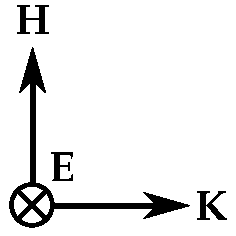
\includegraphics[width=.12\textwidth]{img/tripletHEK.pdf}}
	\end{overpic}
\label{fg_Mie}  \end{figure}

An analytic theory of electromagnetic resonances in dielectric spheres (and cylinders) was developed by Mie in 1908 \cite{mie1908beitrage}, and correspondingly they are denoted as \textit{Mie resonances}. 
Dielectric resonators operate in a similar way to a series L-C circuit, as was noticed by Richtmyer in 1939 \cite{richtmyer1939dielectric}. Few decades later, the dielectric resonator found its use in the developing microwave technology; usually it takes the form of a millimeter-sized ceramics disc glued to the microstrip circuits. 
The Mie theory describes the scattering from a single particle surrounded by vacuum, but for high enough dielectric permittivity $\epsrl \gtrsim 50$, the resonant fields are well confined in the dielectric volume and are not much affected by the presence of the neighbouring cells.
An artificial dielectric consisting of dielectric particles with effective permeability differing from unity was considered by Lewin in 1947 \cite{lewin1947electrical}; apparently it was not until 2002 when O'Brien et al. computed \cite{obrien2002photonic} that the effective permeability of such a structure may be negative.
\label{negn_diel}


Infinite number of the higher-order resonances exist \cite[pp. 407-408]{mie1908beitrage}, resembling the set of single-electron orbitals around an atomic nucleus. Many of these, e.g. most \textit{d}-type orbitals, have zero electric or magnetic dipole moments. Dipole moments of many others exist, but are not oriented parallel to the fields of the incident wave, and do not couple to the electromagnetic wave. In the spectrum of an array of dielectric spheres, one can clearly identify the remaining resonances as the most prominent magnetic one, electric one, the second magnetic, second electric etc. The first three resonances from this alternating series are shown in Fig. \ref{fg_Spheres_lossscan}, each manifesting as a peak in reflectance, and as a pair of resonance in $\meff(f)$ and antiresonance in $\meff(f)$, or vice versa.

%% todo cite vendik, Zhao etc. from the directory

%}}}
\begin{figure}[h!] %fg_Spheres_lossscan %{{{
	\caption{Amplitude of \textbf{(a)} reflectance, \textbf{(b)} transmittance and \textbf{(c)} effective index of refraction $\Neff = \Neff' + \ii \Neff''$ of TiO$_{2}$ spheres with varied loss compared to the natural one from Ref. \cite{baumard1977_epsilon_TiO2}; sphere radius $\rho = 15 \upmu$m, unit cell size $a=100$ $\upmu$m.} \label{fg_Spheres_lossscan} \centering \vspace{-0.030\textwidth} %% TODO
\begin{tabular}{r}
\begin{overpic}[width=0.85\textwidth]{img-meep/Spheres_lossscan_r.pdf}  \put (-1,28) {\textbf{(a)}} \end{overpic}\vspace{-0.060\textwidth}\\
\begin{overpic}[width=0.85\textwidth]{img-meep/Spheres_lossscan_t.pdf}  \put (-1,28) {\textbf{(b)}} \end{overpic}\vspace{-0.060\textwidth}\\
\begin{overpic}[width=0.85\textwidth]{img-meep/Spheres_lossscan_n.pdf}  \put (-1,28) {\textbf{(c)}} \end{overpic}\vspace{-0.060\textwidth}\\ % git add TODO
\begin{overpic}[width=0.87\textwidth]{img-meep/Spheres_lossscan_eps.pdf}\put (-1,28) {\textbf{(d)}} \end{overpic}\vspace{-0.060\textwidth}\\ % git add TODO
\begin{overpic}[width=0.87\textwidth]{img-meep/Spheres_lossscan_mu.pdf} \put (-1,28) {\textbf{(e)}} \end{overpic}\vspace{-8mm}\\ % git add TODO
\end{tabular}
\end{figure}
%}}}
\paragraph{Dielectric losses}%{{{
Unlike split-ring resonators, where the high-frequency dissipative losses depend on many factors such as the eddy currents and details in the geometry, the losses in dielectric resonators are well defined and their effect can be reliably computed by the FDTD simulation. 

We used a realistic model \cite{baumard1977_epsilon_TiO2} of polycrystalline rutile (TiO$_{2}$), according to which the relative permittivity of the spheres was 
$$\epsrl(f = 1\text{ THz}) = 94.2-2.43\text{i}.$$ 
The actual permittivity of the experimentally measured samples depended on their preparation, in particular the volume fraction of microscopic voids. For such composites, Ref. \cite{baumard1977_epsilon_TiO2} gives only the ratio of $\epsrl''/\epsrl'$, but since $\epsrl'$ could be determined from the resonance frequencies in the experimental spectra, also the imaginary part could be easily computed.

The reflectance, transmittance and effective parameters of rutile spheres with radius $\rho=15\;\upmu$m are shown in Fig. \ref{fg_Spheres_lossscan}. Three different levels of losses were considered, with the realistic value represented as 100 \%, and accompanied with a hypothetic low-loss dielectric with 10 \% and 1 \% of original losses. 

The magnetic resonance is located at 530 GHz and the electric one at 790 GHz, the second magnetic resonance follows at 1040 GHz. As a natural result of the Lorentzian model, the dielectric losses grow proportional to the frequency. Notice that around the resonance frequencies, the transmission grows with losses.

Taking realistic losses into account, the curves of the effective parameters in Figs. \ref{fg_Spheres_lossscan}c,d,e become smoother and approach the familiar curve of the damped oscillator in Fig. \ref{fg_oscillator_spectrum}. Strong enough losses prevent the formation of regions with negative effective parameters. Note, however, that formally $\Neff'$ can become negative \cite[pp. 12--15]{pazoutova2011dp} even when either $\eeff'>0$ or $\meff'>0$. Such a negative-index medium is however inevitably extremely lossy, which is represented by its \textit{figure of merit}
\begin{equation} \text{FOM} := \frac{\Neff'(f)}{\Neff''(f)} \lesssim 10. \label{eq_}\end{equation}

At the right hand side of the plot, for $f \sim a/(2c) \approx 1.5$ THz, the structure reaches a Bragg band gap. This kind of resonance is not appreciably affected by the losses, since most of the field energy in the Bragg resonance is concentrated in free space between the particles.

%}}}
\begin{figure}[h!] %% SphereWire_principles %{{{
	\caption{Amplitude of \textbf{(a)} reflectance, \textbf{(b)} transmittance and \textbf{(c)} effective index of refraction $\Neff = \Neff' + \ii \Neff''$ of TiO$_{2}$ spheres, wire grid array, a combined negative-index structure and its modification  with varied loss compared to the natural one from Ref. \cite{baumard1977_epsilon_TiO2}; sphere radius $r = 30 \upmu$m, unit cell size $a=100$ $\upmu$m.} \label{fg_SphereWire_principles} \centering \vspace{-3mm} %% TODO
\begin{tabular}{r}
\begin{overpic}[width=0.85\textwidth]{img-meep/SphereWire_principles_r.pdf}  \put (-1,28) {\textbf{(a)}} \end{overpic}\vspace{-0.055\textwidth}\\
\begin{overpic}[width=0.85\textwidth]{img-meep/SphereWire_principles_t.pdf}  \put (-1,28) {\textbf{(b)}} \end{overpic}\vspace{-0.055\textwidth}\\
\begin{overpic}[width=0.85\textwidth]{img-meep/SphereWire_principles_n.pdf}  \put (-1,28) {\textbf{(c)}} \end{overpic}\vspace{-0.050\textwidth}\\
\begin{overpic}[width=0.85\textwidth]{img-meep/SphereWire_principles_eps.pdf}\put (-1,28) {\textbf{(d)}} \end{overpic}\vspace{-0.050\textwidth}\\
\begin{overpic}[width=0.85\textwidth]{img-meep/SphereWire_principles_mu.pdf} \put (-1,28) {\textbf{(e)}} \end{overpic}\vspace{-0.050\textwidth}\\
\end{tabular}
\end{figure}

%}}}
\paragraph{Negative-index metamaterial based on dielectric spheres} %{{{
An important property of the periodic sphere array is its nearly \textit{isotropic} electromagnetic behaviour, i.e. independence of its behaviour on the wave polarisation. Its roots are in high symmetry of the dielectric sphere, and it is approximately maintained even when the spheres are arranged into a periodic lattice, provided that low frequencies are considered and that the spheres are too close. 
% todo Cai_Zhu2008-Diel_resonators_wires.pdf

Following the approach used to build a metamaterial with a negative refractive index from SRRs, it is possible to interlace the sphere array with the lattice of wires, which introduce negative permittivity. In order to maintain the approximate isotropy of the resulting structure, the wires may be parallel to the $x$- and $y$-axes to form a two-dimensional square mesh. This modification does not make any appreciable change in the low-frequency behaviour. % todo link to the wire mesh simulation

Fig. \ref{fg_SphereWire_principles} compares the already commented spectra for the sphere lattice (red line), and wire grid (blue line) with the spectra for the compound structure, which is sketched in Fig. \ref{fg_spherewire_sketch}a,c. At $f>0$, the wire grid does not reflect all energy, leading again to formation of the Fano resonance lineshapes. 

Notice in \ref{fg_SphereWire_principles} that the Fano resonances of structures with and without the wire mesh have a peculiar complementary shape. The wave reflected from the electric dipole of the wire mesh has an opposite sign than that reflected from the electric dipole of dielectric particles. Its sign determines whether the interference with the second component, scattered by the Mie resonances, would be constructive, or destructive. 

A band of negative index of refraction is formed above the magnetic Mie resonance, between 510 and 550 GHz. When the realistic model of losses in TiO$_2$ is used, the maximum figure of merit $\Neff'/\Neff'' \approx 6$ around the centre of the photonic band. This means that the metamaterial, in the optimum of the negative-index band, reduces the wave amplitude to $e^{1/6} \approx 0.84$ within one wavelength. 

After ca. 40 wavelengths, the amplitude drops to $10^{-3}$ and the wave energy to $10^{-6}$. The applicability of such a metamaterial for building a macroscopic optical device is questionable. % todo \cite{zhao2009mie}

%Another way of achieving negative refractive index is in overlapping the electric and magnetic resonances \cite{holloway2003double} - similar to the el mag resonator above, has low spatial dispersion - but: tight requirements, double losses \cite{zhao2009mie}

%}}}
\paragraph{Effect of elliptic shape}%{{{
For a spherical dielectric particle, the frequencies of the magnetic and electric resonances, $f_{\text{M1}}$ and $f_{\text{E1}}$, respectively, scale inversely proportional to the radius $\rho$:
\begin{equation} f_{\text{M1}} \propto \rho^{-1}, \quad f_{\text{E1}} \propto \rho^{-1}. \label{eq_freq_rho}\end{equation}

When the particle is an ellipsoid with three independent semiaxes $\rho_x$, $\rho_y$ and $\rho_z$ aligned parallel to the $x$-, $y$- and $z$-axes, the resonance frequencies $f_{\text{M1}}$ and $f_{\text{E1}}$ become certain functions of these three ellipsoid parameters. For a nearly spherical shape, 
$$\rho_x \sim \rho_y \sim \rho_z,$$
both frequencies can be approximated as 
\begin{equation}  f_{\text{M1}} \propto \rho_x^{-0.4}  \rho_y^{-0.2} \rho_z^{-0.4}, \label{eq_freqM1_rhoxyz}\end{equation}
\begin{equation}  f_{\text{E1}} \propto \rho_x^{-0.15}  \rho_y^{-0.15} \rho_z^{-0.7}. \label{eq_freqE1_rhoxyz}\end{equation}
Obviously,  in both Eqs. (\ref{eq_freqM1_rhoxyz}) and (\ref{eq_freqE1_rhoxyz}), all three exponents must sum exactly to -1 so that they are compatible with the scaling rule for a sphere in Eq. (\ref{eq_freq_rho}). Their values are approximate only, as they were interpolated from batches of simulations which scanned through the ellipsoid parameters.

When the ellipsoid axes have general orientation, the resonance frequencies remain almost the same; also the resonant modes are  preserved with respect to the ellipsoid orientation. An incident wave in such a case can excite multiple magnetic or electric Mie resonances of the same topology but different orientation, which differ slightly by their frequencies. The structure then may change the polarisation state of the wave, which is beyond the scope of this analysis.

%}}}
\begin{figure}[t]  % fg_spherewire_sketch%{{{
	\caption{Sketch of the sphere array embedded in a wire grid. \texttt{(a)} Front view of the simulated structure, \texttt{(b)} the experimental structure used in Ref. \cite{yakiyama2012terahertz}, measures are in micrometers. \texttt{(c)} and \texttt{(d)} top views of the corresponding structures} \label{fg_spherewire_sketch} \centering 
\begin{overpic}[width=0.30\textwidth]{img/SphereWire_num_xy.pdf} \put (1,81) {\textbf{(a)}}\end{overpic}\quad
\begin{overpic}[width=0.30\textwidth]{img/SphereWire_expe_xy.pdf}  \put (1,81) {\textbf{(b)}}
		\put(100,30){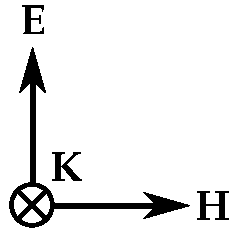
\includegraphics[width=.12\textwidth]{img/tripletEKH.pdf}} % todo
\end{overpic}\quad \\
\begin{overpic}[width=0.30\textwidth]{img/SphereWire_num_xz.pdf} \put (1,61) {\textbf{(c)}}\end{overpic}\quad
\begin{overpic}[width=0.30\textwidth]{img/SphereWire_expe_xz.pdf}  \put (1,61) {\textbf{(d)}}
		\put(100,10){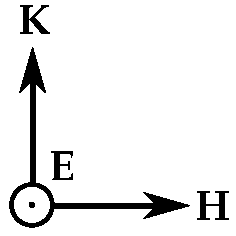
\includegraphics[width=.12\textwidth]{img/tripletKEH.pdf}} % todo
\end{overpic}\quad
\end{figure}

%}}}
\paragraph{Matching simulations and experimental results} %{{{
% approximation for frequency well below the grid resonance  

%}}}
\paragraph{Experimental spectra} %{{{
We performed series of experiments to measure the effective permeability spectrum $\meff(f)$ for a real sample with mean sphere radius of ca. $42\;\upmu$m. The statistical deviation of the resonators size $\sigma \approx 5\;\upmu$m in the sample was determined by means of microscopy and digital image processing. 
%In contrast to simulations, we were able to constraint the spheres' positions to a plane only, while arranging them in a square array appeared unrealistic. 

\begin{figure}[ht]  \caption{Comparison of the effective permeability of ideal monodisperse sphere array (yellow), weighted average according to the size distribution (blue) and experimental data (red dots).}
\label{fg_experimentalConv} \centering 
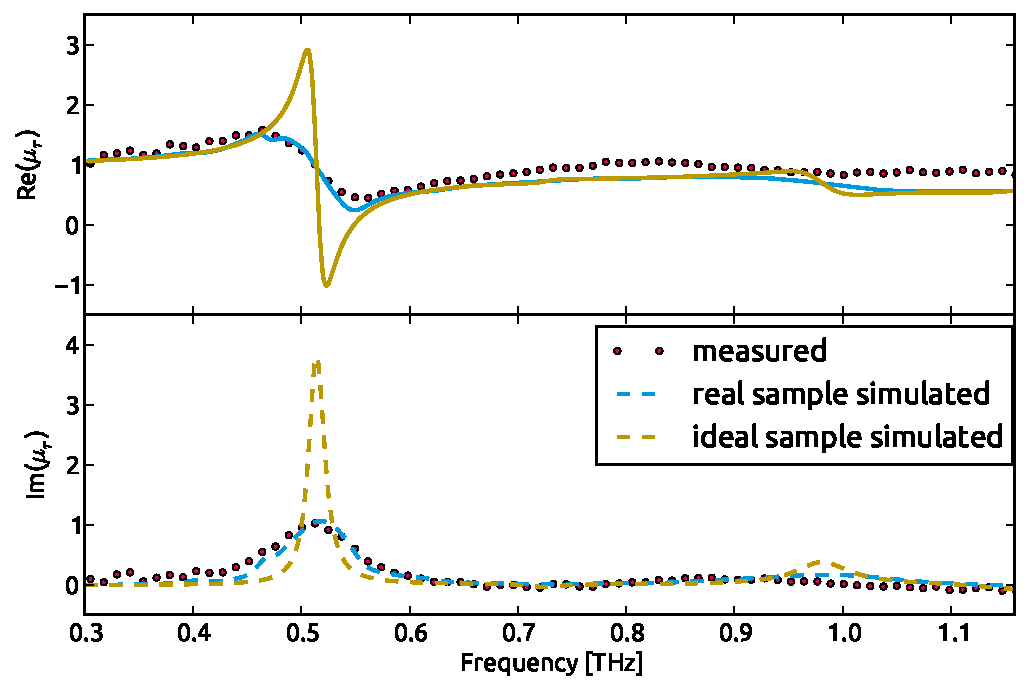
\includegraphics[width=12cm]{img/Spheres_FDTD_experimentalConv.pdf}
\end{figure}

We computed the single-cell permeability spectra (i. e. the yellow curve in Fig. \ref{fg_experimentalConv}) for many different resonator sizes and add them up. The resulting weighted average (blue curve) then matches the experimental data (red dots) nearly exactly. It shall be however noted that the averaged real part of $\mu_{\text{eff}}$ remained positive even with the best sieving results obtained so far. %TODO


%}}}
%   SKIP  \begin{figure}[h] \caption{Current-driven homogenization results for TiO$_2$ spheres %{{{
%    \textbf{(a)} without wires and  \textbf{(b)} embedded in a wire mesh.} \label{fg_cdh3} \centering 
%    	\begin{overpic}[width=.48\textwidth]{img-cdh/cdh_SpheresTiO2.pdf}  \put(1,96) {\textbf{(a)}} \end{overpic}
%    	\begin{overpic}[width=.48\textwidth]{img-cdh/cdh_SpheresLossLess.pdf}  \put(1,96) {\textbf{(b)}} \end{overpic}
%    \end{figure}
%    
%    %}}}
%   SKIP \paragraph{Tunable dielectric resonators} %{{{
%   %TODO Note that the effect of mm-phc transition can be also observed in silicon microcubes (thz operation)
%   %Planar all-silicon metamaterial for terahertz applications \cite{prosvirnin2015planar}
%   
%   %}}}


\FloatBarrier %====================================================================================================
\section{Dielectric rods parallel to the magnetic field} % references to ->
\label{sect_diel_rods_mag}
\add{Such a behaviour at the lower and upper boundaries of the band gap is typical of classical \textit{Bragg} band gaps; individual resonances in other types of structures result in change of $K$ and	introduce more complex differences between the field shape.}
%{{{

analytic shape of the Mie resonance, \cite{obrien2002photonic} 

\add{
 The operation of all sorts of left-handed metamaterials  relies on  the \textit{internal resonances} based on non-propagating evanescent fields in the structure. We conjecture such resonances may never occur in 1-D dielectric structures, so their study requires a simulation of a 2-D or 3-D structure.
% Todo elaborate the idea of nonBragg gap <-> nonradiative fields in structure <-> permittivity/permeability resonance
% Note that in 1-D dielectric PhC, all fields are propagating, none evanesecnt
% Big question: Can one approximate a metamaterial by ENG/DNG/MNG/DPS 1-D PhC??
\begin{figure}[ht] \caption{Dispersion curves for dielectric rods aligned parallel to magnetic field. The side plots show the shape of the fields in the $(x,z)$ plane, at the frequencies of the band edges. The magnetic field is plotted as color map and the electric field is represented by vectors. The rod radius was chosen to 12 \% of the period. \textbf{(a)} On the left, a relatively low permittivity $\varepsilon = 12$ places the magnetic resonance above the first Bragg band gap. \textbf{(b)} For high permittivity dielectric $\varepsilon = 100$, the magnetic resonance forms the first band gap. } \label{fg_rodh} \centering 
\textbf{(a)}	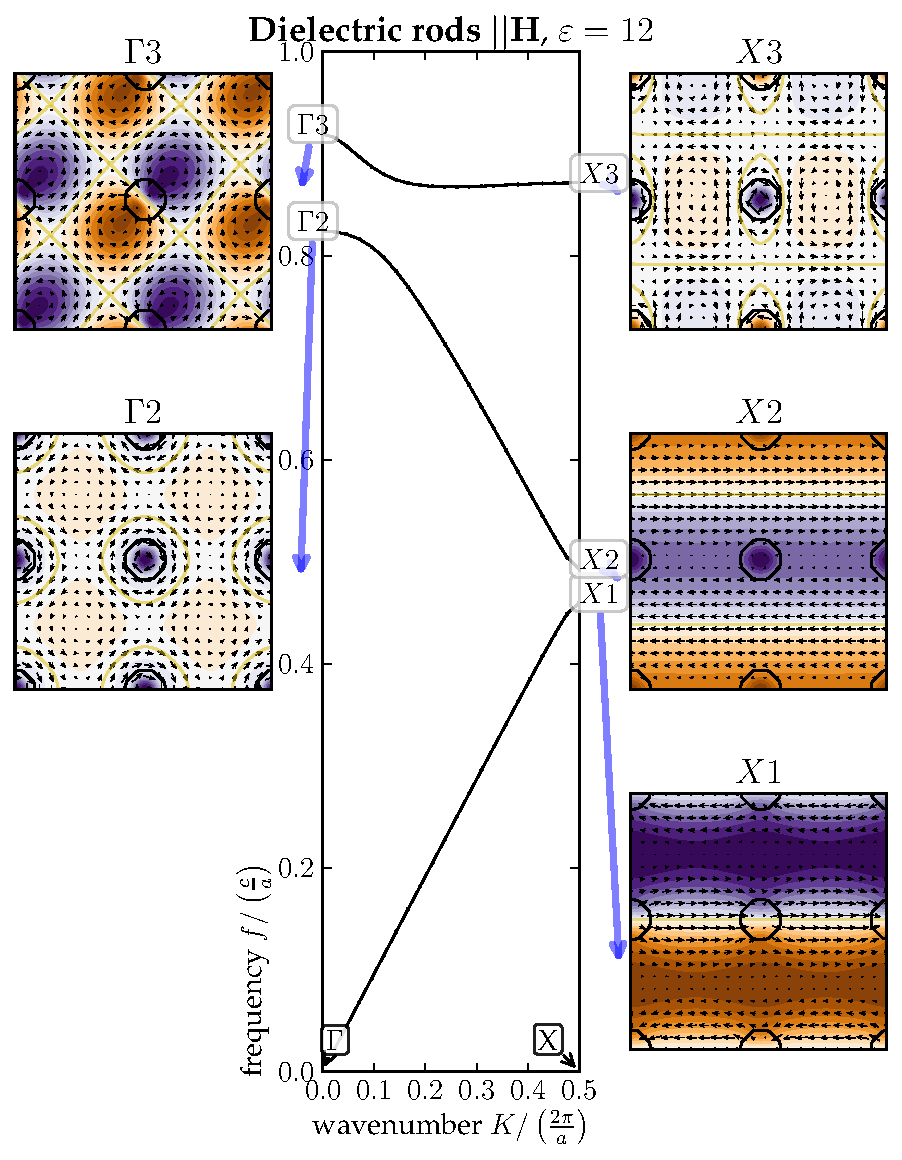
\includegraphics[width=.45\textwidth]{img/HRods_eps012_R12_PWEM.pdf}
\textbf{(b)}	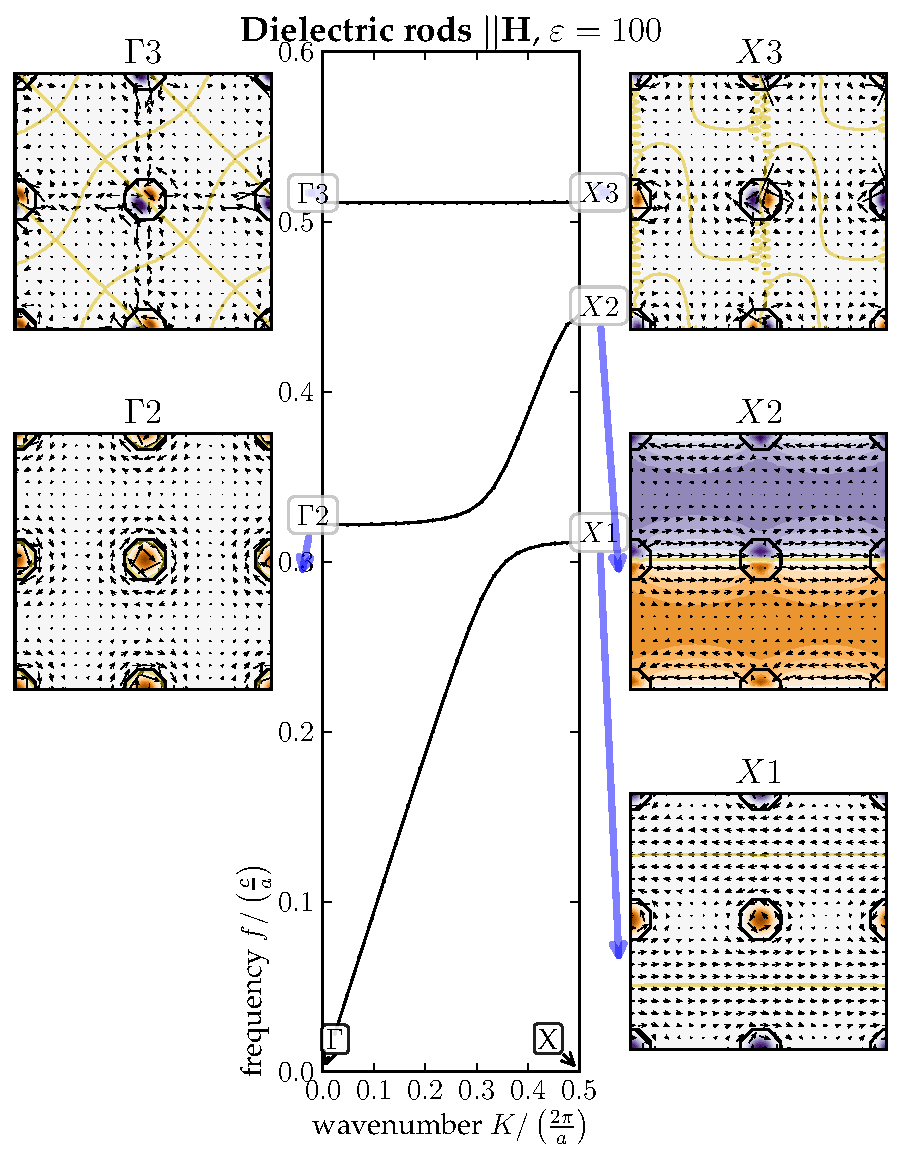
\includegraphics[width=.45\textwidth]{img/HRods_eps100_R12_PWEM.pdf}
\end{figure} %% TODO OVERPIC

Probably the simplest example of such structures is a periodic array of high-permittivity dielectric rods, aligned parallel to the $y$-axis. (We use the convention that the structure is excited by a plane wave source with $\mathbf E || \mathbf x$, $\mathbf H || \mathbf y$ and the wave propagates along the $z$-axis). % dubious - the E, H have many directions in the unit cell; better  to write "TM"/"TE"? But this would confuse with nonperp incidence!
The inhomogeneity of the structure along the $x$-axis allows the electric field to circulate along the rod -- or, more precisely, the $\mathbf E$ field can now be decomposed into purely \textit{planar} part and a purely \textit{circulating} part, that induces a magnetic flux near the rod axis. The circulating electric field is clearly visible on both plots in Fig. \ref{fg_rodh}, where all nonzero components of the fields ($H_y$, $E_x$ and $E_z$) are depicted. 

% discuss why this is not true: each lorentzian introduces delta mu -> so the low-frequency permeability of rod array should be > 1? Attracted to a magnet?
This new type of resonance is known as a \textit{magnetic Mie resonance}, \cite{obrien2002photonic, nemec2009tunable, yahiaoui2009broadband, yahiaoui2011tunable}. Unlike the Bragg gaps, it can be observed also in a single rod in free space. Being a function of the frequency of the incident wave, the magnetic dipole moment of the free-standing dielectric rod follows the characteristic Lorentzian shape of its \textit{resonance curve}. Below the resonance the magnetic dipole moment of the resonator goes to strongly positive values, while in a narrow region above the resonance it is strongly negative. How does this behaviour change if we arrange the rods in an infinite periodic array? 


The results from a PWEM computation are plot in Fig. \ref{fg_rodh}. To obtain comparable dispersion curves in Fig. \ref{fg_rodh_fdtd}, we employed the FDTD simulation and the effective parameter retrieval described above. The main differences are that in Fig. \ref{fg_rodh_fdtd} we plot the frequency $f$ on the horizontal axis and we also use the effective index of refraction $N_{\text{eff}} := K\cdot \frac{c}{2\pi\,f}$ instead of the wavenumber $K$. One advantage of this representation is that $N_{\text{eff}}$ should be compliant with the Kramers-Kronig relations. This criterion always gives \textit{only one} correct solution on how to unfold $K$ to obtain realistic $N_{\text{eff}}$. 
In the simulation, the rod spacing (or, lattice constant) $a$ was 100 $\upmu$m, so the normalised frequency unit is $c/a = 3$ THz. The frequency range from 0 to 1.8 THz was therefore chosen the same as in Fig. \ref{fg_rodh}b. 
Note the first resonance shows pronounced resonant shape in the plot of permeability, which is typical of magnetic Mie resonances. In a very narrow region 960-970 GHz, the permeability $\mu_{\text{eff}}$ is real and negative. 
Apart from $N_{\text{eff}}$, the FDTD computation gives also the effective wave impedance $Z_{\text{eff}}$, which is a complementary information we need to compute the effective permittivity $\varepsilon_{\text{eff}}$ and the effective permeability $\mu_{\text{eff}}$:

\begin{equation} \varepsilon_{\text{eff}} = N_{\text{eff}}/Z_{\text{eff}}, \quad\quad\quad\quad \mu_{\text{eff}} = N_{\text{eff}}\cdot Z_{\text{eff}}.
\label{eq_epsmu}\end{equation}

\begin{figure}[ht]  \caption{Effective parameters of an array of dielectric rods $||\mathbf H$ with same parameters as in Fig. \ref{fg_rodh}b (i.e. radius of  12 \% of the period and permittivity $\varepsilon = 100$). Complex reflection $r$ and transmission $t$ spectra allow to compute the effective index of refraction, impedance (not shown), permittivity and permeability. Thin grey lines indicate the Brillouin zone boundaries.}
\label{fg_rodh_fdtd} \centering 
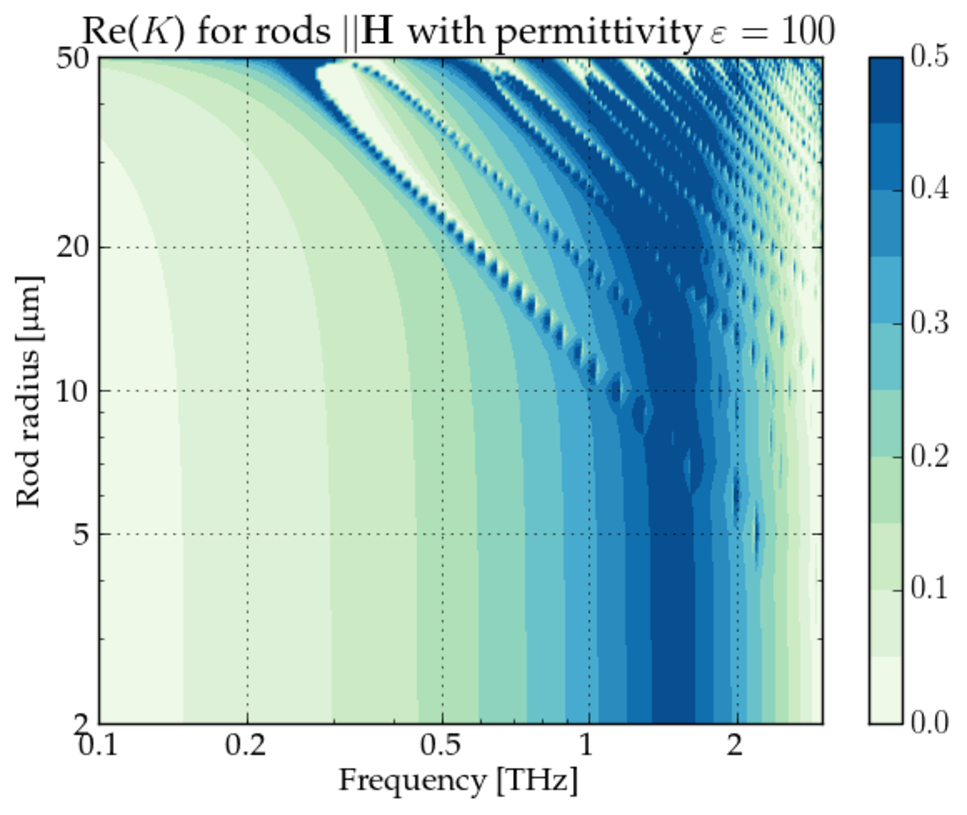
\includegraphics[width=8cm]{img/old/HRods_eps100_radiusscan.pdf}
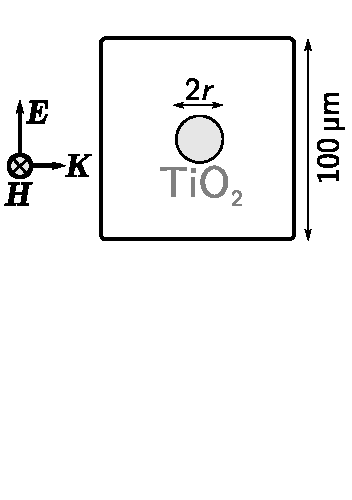
\includegraphics[width=4.5cm]{img/HRods_sketch.pdf}
\end{figure}


The frequency of the Mie resonances is not significantly influenced by the photonic bands. Therefore, in order to understand the resulting band structure and its dependence on parameters, one has to disentangle which band gaps are due to Bragg reflection and which correspond to magnetic or electric Mie resonances. This is much easier knowing the spectra of $\varepsilon_{\text{eff}}$ and $\mu_{\text{eff}}$, as provided by FDTD in Fig. \ref{fg_rodh_fdtd}.
\begin{figure}[ht] \caption{The spectra of the wavenumber $K$ for different rod radii and two different rod permittivities. The wavenumber plot is folded so it ranges from 0 to 0.5, where $K\approx 0$ and $K\approx 0.5$ correspond to band gaps. \textbf{(a)} Medium-permittivity rods with $\varepsilon = 12$, \textbf{(b)} high-permittivity rods with $\varepsilon = 100$.  } \label{fg_hbar_radiusscan} \centering 
\textbf{(a)}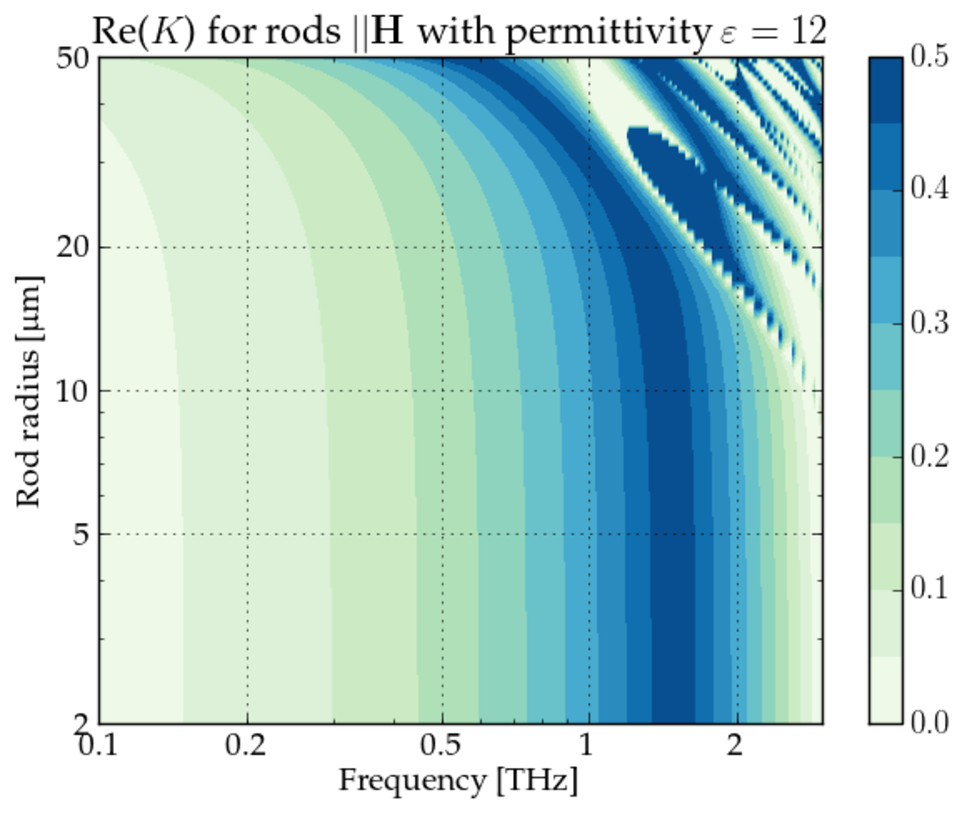
\includegraphics[width=8cm]{img/old/HRods_eps012_radiusscan.pdf}
\textbf{(b)}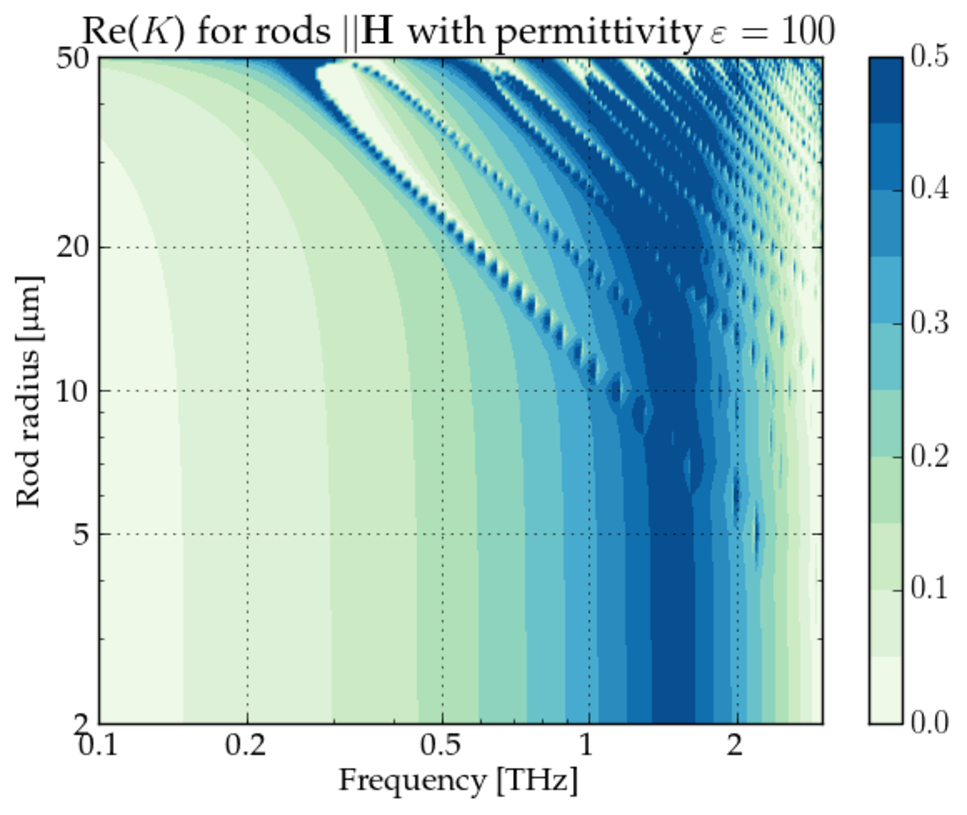
\includegraphics[width=8cm]{img/old/HRods_eps100_radiusscan.pdf}
\end{figure}

The photonic crystals composed of square lattice of dielectric rods have been examined thoroughly since early 90s \cite{plihal1991two, pendry1992_transfer_matrix}. The permittivity of the constituent materials was rather low, corresponding to the optical or near-infrared frequencies, where the suitable materials usually have permittivity $\varepsilon < 12$. By parametric scans we could prove that for rod permittivity below 60 or even 80, the individual resonance is always located at higher frequency than the Bragg gap. Little, if any, attention was therefore paid to different nature of the higher resonances and most publications focused on properties and applications of the Bragg band gap.

The situation is different in the terahertz range, as the lattice of the crystalline solids often exhibits optical phonons at frequencies between 5 and 20 THz. The permittivity of many materials turns out to be much higher for frequencies below these resonances. This enables to conceive structures composed e.g. of titanium dioxide \cite{baumard1977_epsilon_TiO2} with $\varepsilon^{\text{THz}} \approx 92$ or of ferroelectrics with $\varepsilon^{\text{THz}}$ even orders of magnitude higher \cite{skoromets2011tuning}. The price to be paid for this advantage in the THz range are the relatively high losses caused by the lattice vibrations.

\begin{figure}[ht] \caption{Behaviour of the rods $||\mathbf E$, with permittivity $\varepsilon = 100$ and radius $r=11\;\upmu$m.\\
\textbf{(a)} Band diagram and modes from PWEM. 
} \label{fg_erod_radius11} \centering 
\textbf{(a)}	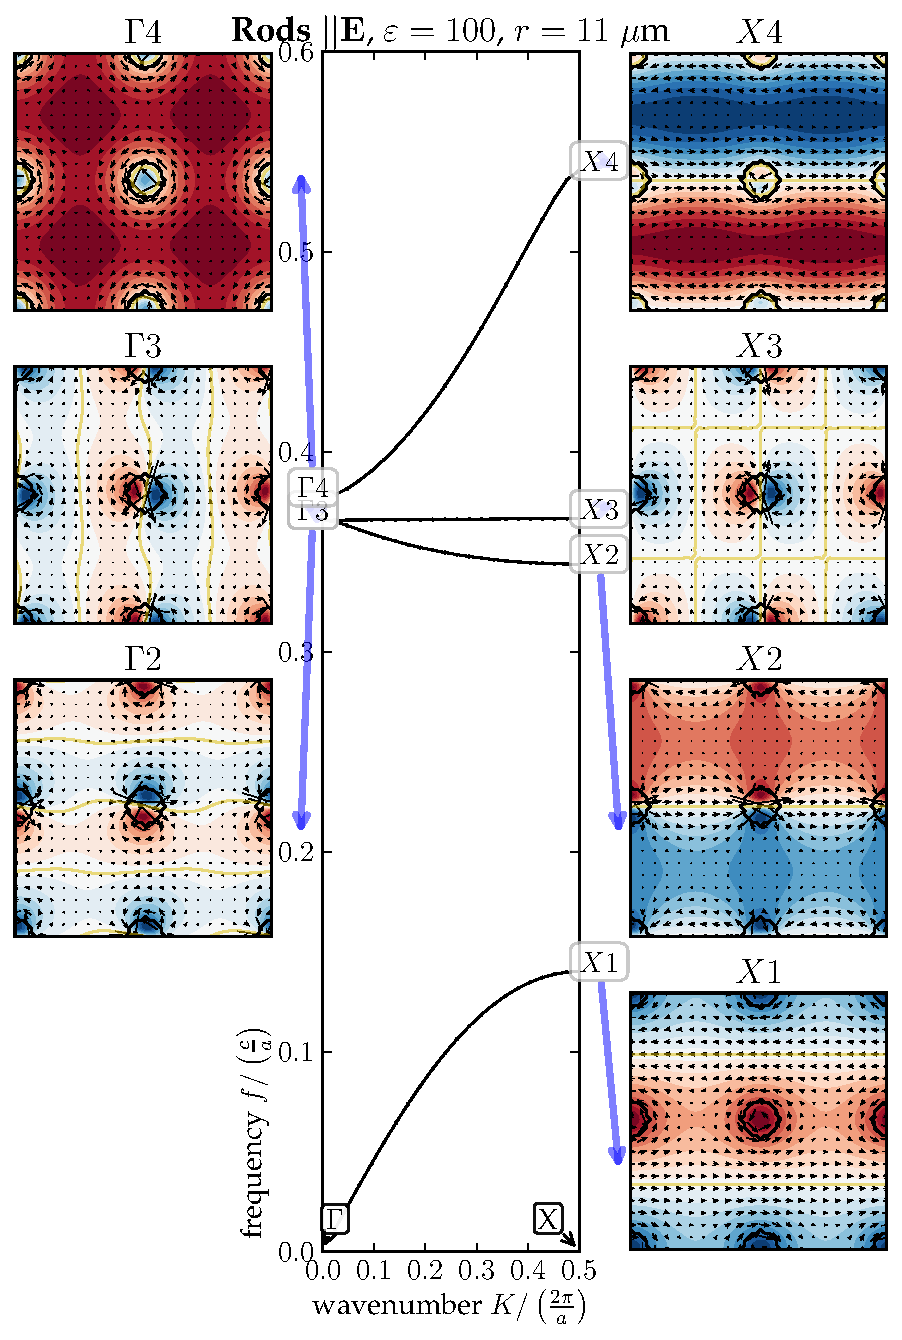
\includegraphics[width=8.5cm]{img/ERods_eps100_R11_PWEM.pdf}
\end{figure}

}

%}}}





\FloatBarrier %====================================================================================================
\section{Dielectric rods parallel to the electric field} % references to ->

\label{sect_diel_rods_el}
%{{{
% TODO refereence  also to \cite{valdivia2012} and \cite{shi2007}
\cite{yang2015}




%}}}

%{{{ FROM SHORT.pdf
\mdf{  
\begin{figure}[ht] \caption{The spectra of the wavenumber $K$ for different rod radii and two different rod permittivities, analogical to Fig. \ref{fg_hbar_radiusscan} except for different orientation. \textbf{(a)} Medium-permittivity rods with $\varepsilon = 12$, \textbf{(b)} high-permittivity rods with $\varepsilon = 100$.  } \label{fg_ebar_radiusscan} \centering 
\textbf{(a)}	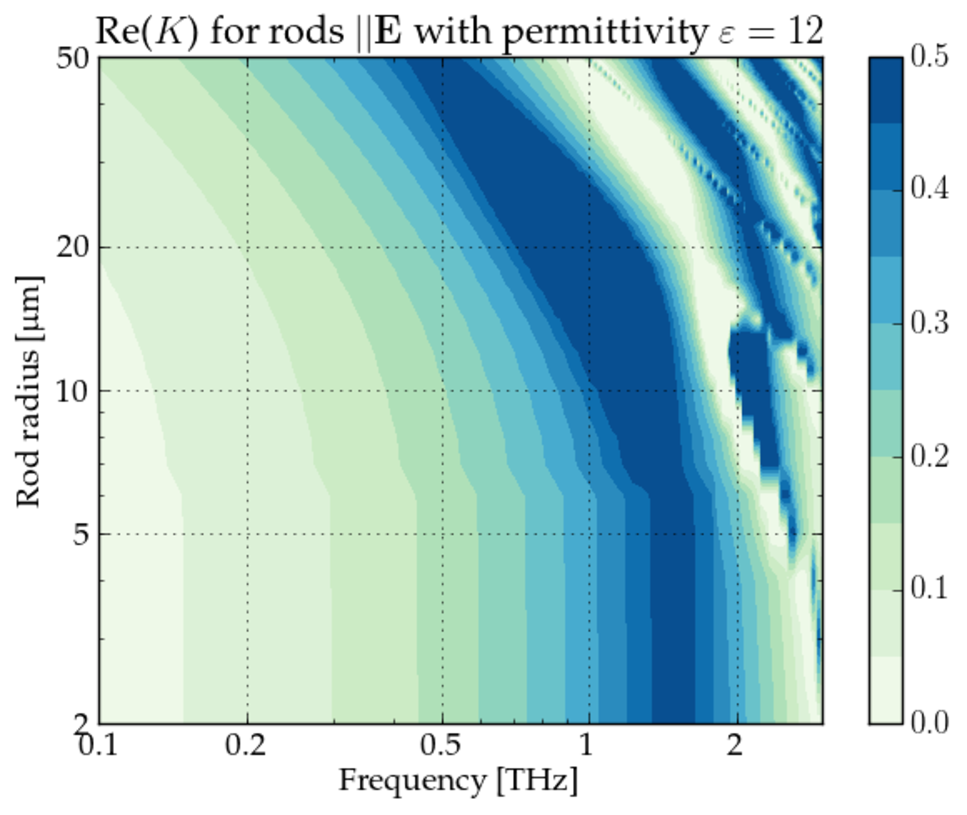
\includegraphics[width=8cm]{img/old/ERods_eps012_radiusscan.pdf}
\textbf{(b)}	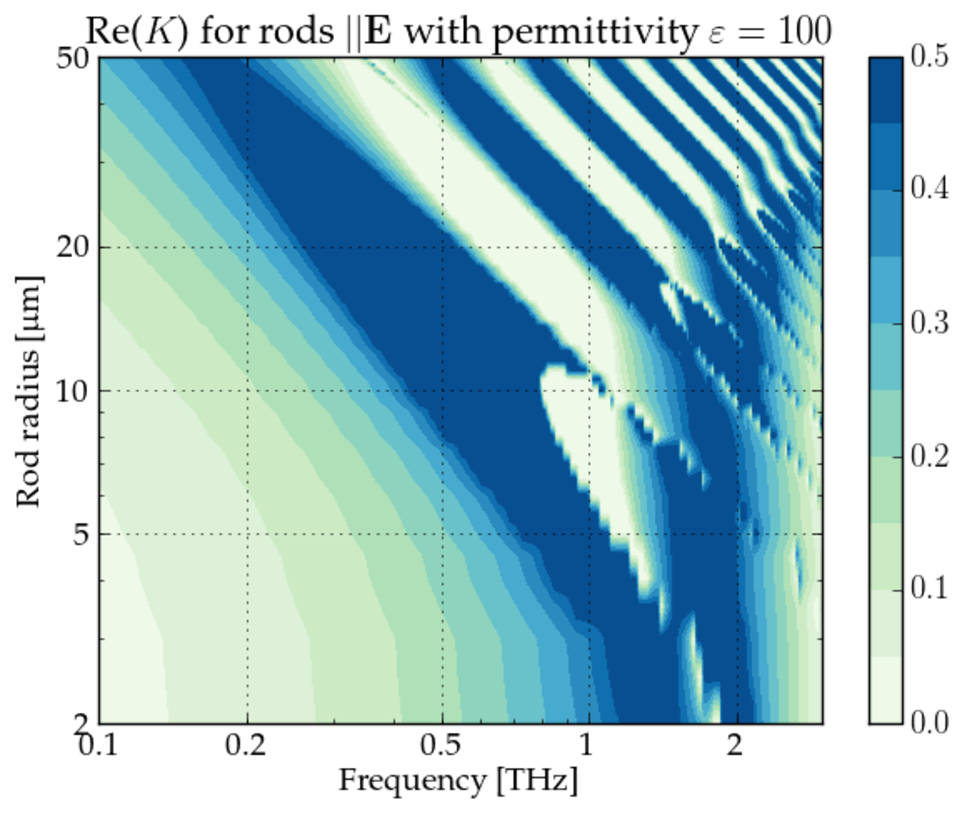
\includegraphics[width=8cm]{img/old/ERods_eps100_radiusscan.pdf}
\end{figure}


The dielectric bars parallel to the electric field represent the same structure as previously discussed, except that it is orthogonally rotated. There is however a qualitative difference in that the high-permittivity dielectric is continuous along the direction of the electric field, so the effect of the dielectric is expected to be much stronger. This results in that the first Mie resonance is the \textit{electric} one. Its overlap with the next magnetic resonance can eventually lead to negative index of refraction in such a structure \cite{peng2007, vynck2009all}. If the permittivity of the rods is chosen to be $\varepsilon = 100$ and the periodicity of the lattice $a = 100\;\upmu$m, the negative index of refraction occurs in a narrow range of radii from 9 to 12 $\upmu$m. The behaviour of this structure with the desired radius is depicted in Fig. \ref{fg_erod_radius11}a,b.

In order to form a photonic band with a negative index of refraction, both the permittivity and permeability need to be negative. In the structure discussed, this is made possible by the frequencies of the electric and magnetic Mie resonances being close enough to overlap.
The electric resonance would be surrounded by its broad band gap between the frequencies spanning from $0.13 \cdot\frac{c}{100\;\upmu\text{m}} \approx 400$ GHz to  $0.38 \cdot\frac{c}{100\;\upmu\text{m}} \approx 1140$ GHz. This is also confirmed by Fig. \ref{fg_erod_radius11}a where the mode shapes X1 and $\Gamma$4 perfectly correspond to the electric Mie resonance. 

For the interesting range of radii around 11 $\upmu$m, the magnetic resonance introduces a new, narrow photonic band starting from X2. Now, moving on to the right plot of Fig. \ref{fg_erod_radius11}b, we can clearly identify the resonant frequencies of 815 and 900 GHz. They cause abrupt skips of the refractive index which always shift the index of refraction by one Brillouin zone down.\footnote{The individual resonance appears to be the only mechanism that causes $N'_{\text{eff}}$ to \textit{decrease} in the spectrum. In photonic bands, no matter if $N_{\text{eff}} > 0$  or $N_{\text{eff}} < 0$, the real part of $N_{\text{eff}}$ always grows in accordance with the Foster theorem. This is confirmed by the FDTD results and by their compliance to Kramers-Kronig relations. To illustrate this, the Hilbert transform of the refractive index is plotted as the thin pink line and it nearly perfectly follows the green curve over whole spectrum, except for an additive constant. There is  only one acceptable physical solution that is compatible with the Kramers-Kronig relations.}
The resonance is accompanied by a sharp peak in the imaginary part of refractive index $N''$ and by transmission amplitude touching zero ($|t| = 0$). As both Mie resonances precede the Bragg gap, the index of refraction is pushed into negative values and the following photonic band gap $N' < 0$.

For completeness we add the FDTD results with effective permittivity and permeability, computed for the entire spectrum. These quantities however seem to have a useful physical interpretation only within the photonic bands, or within those parts of the photonic band gaps where $N = 0$. 
\\

The dispersion curves of the rods with radii different than 11 $\upmu$m are compared in Fig. \ref{fg_ebar_radiusscan}b based on multiple FDTD simulations. The individual resonances are again easy to be distinguished by abrupt changes from white to blue or vice versa (i.e. skips between the Brillouin zones). We can see that for radii below 8 $\upmu$m the magnetic resonance is at too high frequencies, forming its separate band gap. For even thinner rods at the very bottom edge of the plot, no individual resonance intersects with the first Bragg  band gap at all. 

An interesting qualitative change of the structure response occurs when the rods get slightly thicker than discussed above, say $r > 12\;\upmu$m. The electric and magnetic resonance frequencies do never cross over, but instead they  and an ordinary Bragg band gap remains. The transmission curve of single cell (Fig. \ref{fg_erod_radius11}) continuously shifts up and does not touch zero anymore. We may conclude that for rod radius being too high, the structure no more exhibits the negative index of refraction and starts to behave similar to the 1-D photonic crystal discussed above.
% TODO explanation by nodal planes

%The dependence of the folded wavenumber $\text{Re}(K)$ for high-permittivity rods $||\mathbf E$ is plotted in Fig. \ref{fg_ebar_radiusscan}b. Starting from very thin rods ($r=2$ \um) at the very bottom of the plot, we can see the first band gap (1.3 to 1.5 THz) denoted by darkest blue is purely of the Bragg type, followed by a 

Comparing the low-permittivity and high-permittivity cases in Fig. \ref{fg_ebar_radiusscan}a,b, one can see there exists some minimum limit for the permittivity contrast that is necessary for both electric and magnetic resonances to be located in the first gap simultaneously. We determined this scale-invariant value to be roughly 80.

The transmission peaks can be clearly identified with resonant modes and it was observed that the frequencies of the modes shift with different slope depending on parameters.  
} 
%}}}




\begin{figure} \centering 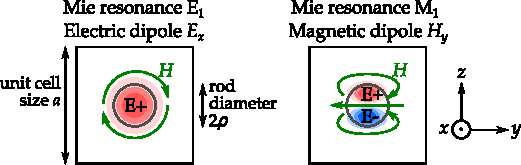
\includegraphics[width=14cm]{img/ERods_1st_and_2nd_Mie_resonance.pdf}%{{{
\caption{(a) Perspective view of the unit cell\add{; (b) its} cross-sections with the resonant modes excited by a plane wave with $\mathbf{E}||x, \mathbf{H}||y$ and $\mathbf{k}||z$. The first Mie resonance has an electric dipole moment only, while the second one has a magnetic dipole moment instead. The red and blue color shows positive and negative values of the $E_x$ component of the electric field, while the magnetic field is represented by the arrows. } \label{fg_sketchfield} \end{figure}

Our structure \add{(see Fig.\ref{fg_sketchfield}a)} is defined by a square unit cell with the linear dimension $a$ periodically distributed in the $yz$ plane; the dielectric rod parallel to $x$-axis with radius $\rho$ and permittivity $\varepsilon_r$ is positioned in its center. We employed the finite-difference time-domain (FDTD) simulation package MEEP \cite{oskooi2010meep} to obtain the scattering coefficients (complex reflectance $r$ and transmittance $t$) of a structure with variable number of unit cells along the wave vector direction $k\parallel z$. The incident wave is polarized $E\parallel x$, periodic boundary conditions were applied in the $y$-direction. We performed the simulations for a single layer ($y$-periodic boundary conditions only). Its effective properties are almost identical to those of the corresponding multilayer structure. We checked that for this geometry, the retrieved effective parameters depend only negligibly on the number of unit cells in the $z$-direction. The relevance of the calculations with a single layer was further confirmed by current-driven homogenization simulations \cite{markel2013current} in several particular cases (same geometries as in Fig.~\ref{fg_spec}) which yielded a response in a very good agreement with the FDTD results.

The effective parameters were \add{then} retrieved from complex transmittance and reflectance spectra \cite{smith2002determination}.  \add{Alternative means of obtaining the effective parameters are discussed in Ref. \cite{simovski2009material}. When inverting the Fresnel-Airy formulas, the correct solutions have to be chosen in the different parts of the $\Neff(\omega)$, $\Zeff(\omega)$ spectra \cite{simovski2009material}; to this aim, Kramers-Kronig relations as well as the conditions of a passive medium Im$(\Neff)>0$ and Re$(\Zeff)>0$ were used.} 

The retrieved value of the complex effective index of refraction $\Neff(f)$ defines the magnitude of the wave vector
\begin{equation}\label{eq_wave_vector} k(f) = 2\pi f \Neff(f) /c\,.  \end{equation}
Note that the retrieval procedure  implies that the wave vector introduced by Eq. (\ref{eq_wave_vector}) is defined in an unfolded reciprocal space. 

A Bragg resonance occurs when an integer number of half-wavelengths fit into one unit cell, i.e.,  when
\begin{equation}\label{eq_BZ} k(f) = \frac{q \pi}{a}\,, \end{equation}
where $q$ is a non-zero integer. In such a situation, the wave vector is located at a Brillouin zone boundary. The purely real values of $k$ then describe photonic band edges.  In a band edge state, a standing wave appears in the structure and it is characterized by exactly $q$ nodal planes dividing each unit cell in the transverse direction to $q+1$ disconnected parts. The band edges delimit a photonic {\itshape Bragg band gap} where only evanescent waves described by $\Neff''>0$ can exist.  We can write an equation analogous to (\ref{eq_BZ}) for the real part of the refractive index:
\begin{equation}\label{eq_BZN} \Neff'(f) = \frac{q c}{2 a f}\,; \end{equation}
its hyperbolic behavior versus frequency reflects the pinning of the wave vector to the Brillouin zone boundary inside the Bragg band gap.

Another case of interest where evanescent waves are obtained is that of $\Neff' = 0$ (center of the first Brillouin zone, $q=0$) and $\Neff''>0$. Here the waves exponentially decay in the medium without any phase change. However, this behavior has a different origin: it is connected to a plasma-like response of the material ($\varepsilon<0$ or $\mu<0$) and in this paper we use the term \textit{plasma band gap} to refer to it.

The Kramers-Kronig relations require that for any structure studied, $\Neff'(f)$ [or, equivalently, $k(f)$] attains and finally crosses the Brillouin-zone boundaries when the frequency is sufficiently increased. While usually the convention is used that the corresponding curves are folded back into the first Brillouin zone, in this paper we plot $\Neff'(f)$ in the original (unfolded) Brillouin zones resulting from the retrieval algorithm. This can be clearly observed on the dispersion of the refractive index in Fig.\ \ref{fg_spec}. In this way we retain the information about the number of the nodal planes intersecting the unit cell, which is important for our discussion.
%}}}

\todo{FIGURE: Results of the FDTD simulations for a single layer of dielectric rods with $\varepsilon_{\rm r}= 100$, $\rho=10$\,$\upmu$m. The spectra of reflection $|r|$ and transmission $|t|$ amplitudes share their frequency axes with the retrieved complex effective index of refraction $\Neff$, permittivity $\eeff$ and permeability $\meff$, whose imaginary parts are denoted by dashed lines. The frequency ranges where $\eeff$ and $\meff$ have no physical interpretation (Bragg band gaps or higher order photonic bands) are gray shaded.  } 

In the following, we first describe in detail three characteristic cases: we compare the effective parameters computed for three slightly different unit-cell sizes while the rod radius and the dielectric permittivity are fixed. The comparison of these cases reveals quite remarkable changes in the optical behavior of the structure. We then complement this comparison by a continuous scan of the unit-cell sizes in order to obtain an overview of all possible types of the response for the rod-based geometry.  

In Fig.~\ref{fg_spec}, we show the calculated reflectance and transmittance amplitude spectra, as well as the effective parameters of three representative structures which have the same rod radii $\rho = 10$~$\upmu$m, but they differ by the unit-cell size $a =$ 120, 100 and 80 $\upmu$m. These values of $a$ were selected to illustrate three qualitatively different regimes of behavior.  The dielectric was defined by a simple lossy model with one high-frequency oscillator, its  permittivity was $\varepsilon_r = 100.1 + 0.5\mathrm{i}$ at 500 GHz.

%}}}
\paragraph{Sparse array} %{{{
In Fig.~\ref{fg_spec}(a), where the unit-cell size $a=120$~$\upmu$m, we can see two well separated Mie resonances: the electric one at 680 GHz and the magnetic one at 1030 GHz.  The field distribution of the corresponding modes is sketched in Fig.~\ref{fg_sketchfield}. The resonance frequencies can be easily identified by an abrupt drop in the real part of the effective index of refraction $\Neff'$, accompanied by a sharp peak in its imaginary part $\Neff''$. The Mie resonances in periodic media without losses must always be adjacent to a Bragg band gap. For instance, in Fig.~\ref{fg_spec}(a) at frequencies below the first Bragg gap, the electric dipoles within each rod are directed along the electric field in the rest of the unit cell. The rods thus positively contribute to the refractive index $\Neff'$ which progressively grows until it reaches the first Brillouin zone boundary. At this point, the Bragg condition for a photonic band-gap is fulfilled and each unit cell is intersected by one nodal plane. This is reflected by the dispersion of $\Neff'(f)$ which follows the first Brillouin-zone boundary in the first Bragg band gap between 400 and 680\,GHz [equivalent to $q=1$ in Eq. (\ref{eq_BZN})]: $$	\Neff'(f) = \frac{c}{2af}\,. $$ At 680\,GHz, the electric Mie resonance occurs which dramatically changes the near-field photonic properties of the structure. The observed drop in $\Neff'(f)$ and the slope change in $\Neff''(f)$ mark the plasma-like character of the adjacent part of the band gap which extends up to the plasma frequency of the Mie resonance (940\,GHz). In this frequency range the electric dipoles in the rods change their direction and induce an electric field opposite to the incident one.

For this sparse array of dielectric rods, the first magnetic Mie resonance lies at 1030\,GHz, above the plasma frequency of the electric mode.  The second Bragg band-gap opens at 1010 GHz and, due to the Mie resonance, it is transformed to a plasma band gap at 1030 GHz. The next allowed photonic band starts above magnetic plasma frequencies at 1070 GHz. Therefore we observe a very analogous behavior near the magnetic resonance. 

For completeness we note that at 1350 GHz, a third Bragg band gap starts which, unlike the lower-frequency ones, does not contain any Mie resonances [see Fig.\ \ref{fg_spec}(a)].

The resonances in the effective permittivity $\eeff=\Neff/\Zeff$ and permeability $\meff = \Neff\cdot \Zeff$ of a periodic array obviously exhibit shapes very different from the well-known resonance curves of a damped oscillator \cite{koschny2003resonant}. In the two separate plasma band gaps we obtain either $\eeff < 0$ or $\meff<0$, i.e. the usual behavior observed in the reststrahlen bands of resonances. However, in the Bragg band gaps occurring just below these spectral ranges the behavior of $\eeff$ and $\meff$ does not have any useful physical interpretation and it can be understood as a purely formal frequency dependence: we shaded these ranges with light gray in Fig.~\ref{fg_spec}.
%}}}
\paragraph{Medium array}%{{{
When the unit cell size is reduced to $a=100$~$\upmu$m, as depicted in Fig.~\ref{fg_spec}(b), the Mie resonances shift slightly. Interestingly, in comparison with the sparse array, the electric resonance frequency increases from 680 to 780 GHz, and that of the magnetic resonance decreases from 1030 to 980 GHz. This can be explained by the inter-cell coupling: the circulating magnetic field of the first resonance is compressed when the rods get closer, whereas the magnetic dipoles of the second resonance can couple more easily to each other in the same situation (see Fig.~\ref{fg_sketchfield}).

The converging of the resonance frequencies is linked to the most important qualitative change in the spectra: the fact that the magnetic resonance occurs at a frequency where $\eeff'<0$. The first band gap (the lowest continuous frequency region where $\Neff''>0$) is thus composed of three adjacent regimes: the first Bragg band gap (425--780 GHz), a plasma band gap (780--980 GHz) and the second Bragg band gap (980--1020 GHz). Every Mie resonance introduces a drop in $\Neff'$, so the following photonic band (1020--1070 GHz) features a negative index of refraction ($\Neff'<0; \Neff''\approx 0$), i.e., the phase and group velocities are opposite to each other. We conjecture that the presence of two Mie resonances in the \textit{first} combined band gap is a necessary and sufficient condition for $\Neff'<0$ to occur.

Note that the transmittance amplitude reaches quite small values between the Mie resonances when they are sufficiently close to each other [Fig. \ref{fg_spec}(b)]. This range forms a well-defined band with a reflectance-to-transmittance contrast much better than that observed in a planar Fabry-Perot resonator. One layer of dielectric rods with proper parameters can therefore be applied as a thin, yet very effective filter.
%}}}
\paragraph{Dense array}%{{{
Perhaps an even more surprising change occurs when the rod spacing is further reduced. The Mie resonances get even closer in the spectrum and eventually they vanish for $a=80$~$\upmu$m [see Fig.~\ref{fg_spec}(c)]. The band gap remains at nearly the same spectral position as in panel (b) of this figure, but, unlike for the medium array, the value of $\Neff'$ does not drop within the Bragg band gap. In contrast, it is shifted up to the second Brillouin zone boundary where it meets the second Bragg band gap as clearly seen in panel (c), indicating that each unit cell is intersected by two nodal planes in this state.

The reason of this behavior is related to the change of the nodal plane topology caused by the inter-cell coupling. When the rods are far from each other ($a\gtrsim 100$~$\upmu$m), the individual Mie resonances create closed regions delimited by a nodal surface where the fields are opposite to the rest of the unit cell. Upon reducing the unit-cell size ($a\lesssim 80$~$\upmu$m), the regions of opposite fields start to overlap with those from the neighboring cells and the corresponding nodal surfaces interconnect and open. This pair of open nodal surfaces dividing the unit cell manifests itself by a qualitative change of the $\Neff'$ spectrum towards a shape typical for one-dimensional photonic crystals.

\begin{figure}\centering 
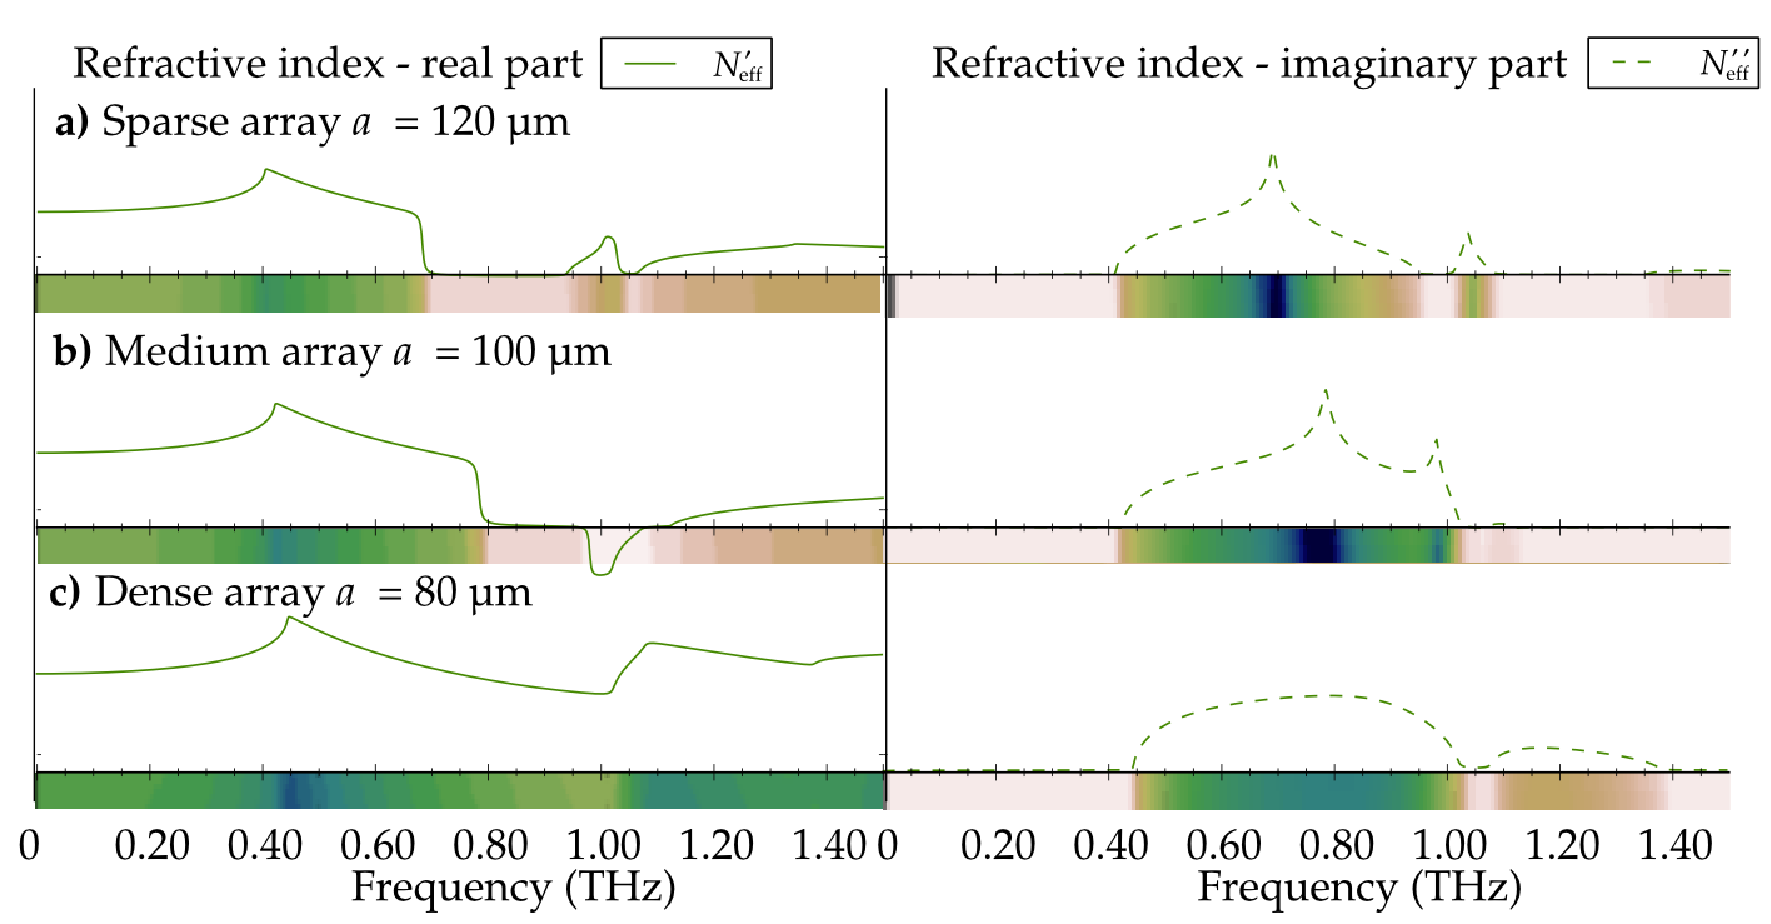
\includegraphics[width=0.5\textwidth]{img/ERods_sketch_of_separate_spectra_to_continuous_scan.pdf}
\caption{} \label{fg_spacingscan100formation}. 
\end{figure}



\begin{figure}\centering  %% TODO rename Re<--->Im
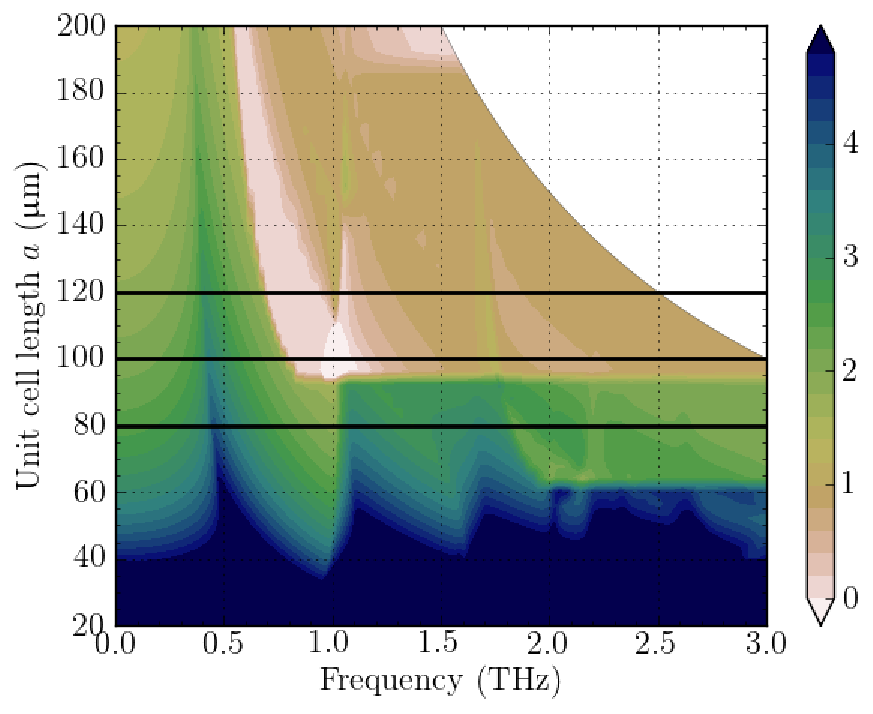
\includegraphics[width=0.5\textwidth]{img/ERods_eps100_spacingscan_Nim.pdf}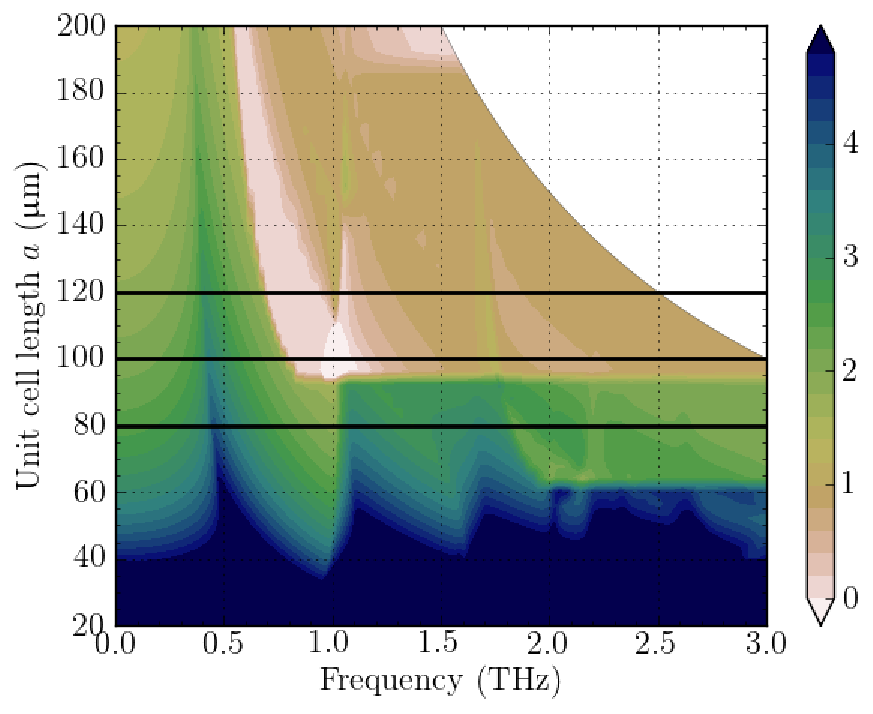
\includegraphics[width=0.5\textwidth]{img/ERods_eps100_spacingscan_Nre.pdf}
\caption{Real ($\Neff'$, left panel) and imaginary ($\Neff''$, right panel) parts of the refractive index for a dielectric rod array with permittivity $\varepsilon_r =100$, radius $\rho = 10$ $\upmu$m and a variable unit cell size $20\:\upmu$m $<a<200\:\upmu$m.  The three solid horizontal lines correspond to the values used in Fig.~\ref{fg_spec}.}
\label{fg_spacingscan100}. 
\end{figure}
%}}}

\paragraph{Continuous scan of the unit-cell size}%{{{
The behavior described above is confirmed by the plots of the complex index of refraction $\Neff',\: \Neff''$ for a continuously varying unit cell size $a$ from 20 to 200~$\upmu$m (Fig.~\ref{fg_spacingscan100}). Here, again, the constant values of the dielectric permittivity $\varepsilon_r=100$ and the rod radius $\rho=10$ $\upmu$m are used. In the upper-right corner of both plots, for $a>c/f$, an empty area is left where the diffraction precludes the determination of effective parameters. 

For an easier interpretation of the results, we draw the most prominent features schematically in Fig.~\ref{fg_drawn100}. Some of them are common in ordinary one-dimensional photonic crystals, namely, the photonic (Bragg) band gaps which are painted in color in Fig.~\ref{fg_drawn100}.

\begin{figure}
    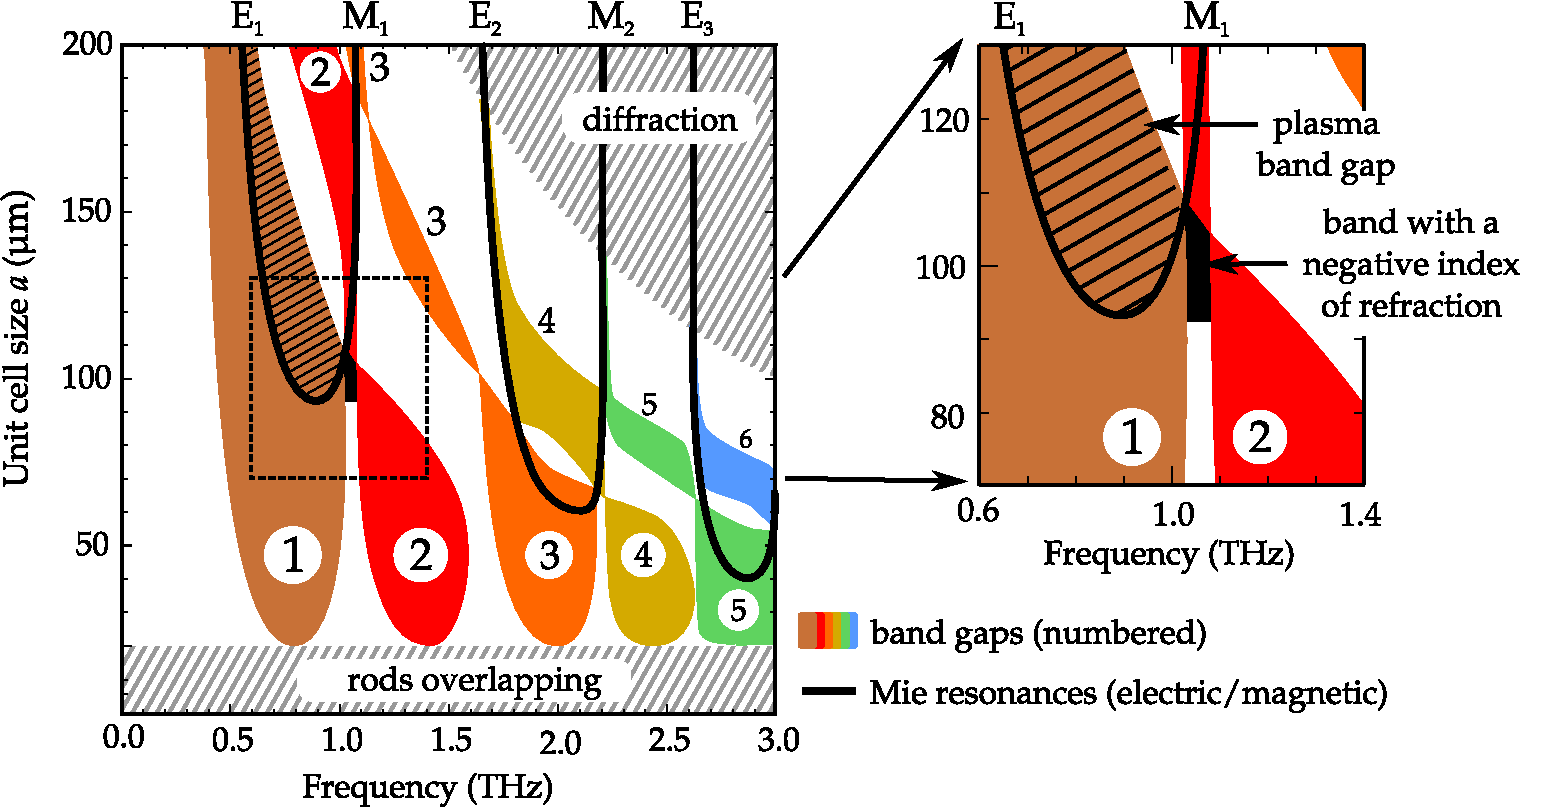
\includegraphics[width=15cm]{img/ERods_eps100_spacingscan_drawn_bands.pdf}
    \caption{Scheme of band gaps and Mie resonances under the same conditions as
    in Fig.~\ref{fg_spacingscan100}.}
\label{fg_drawn100}
\end{figure}




The Mie resonances are caused by the field confinement near the high permittivity elements. They always manifest themselves as sharp peaks in the imaginary part of the index of refraction ($\Neff''$), and in Fig.~\ref{fg_drawn100} they are denoted by thick solid curves. Their electric- or magnetic-dipole character is identified by the letters "E" or "M" above the plot, respectively.

As it can be seen in Figs.~\ref{fg_spacingscan100} and \ref{fg_drawn100}, the pairs of electric and magnetic Mie resonances form U-shaped curves, at the bottom of which the resonances come closer in frequency to each other and eventually they disappear when the unit-cell size $a$ is further reduced. The resonances influence the whole spectra of the refractive index $\Neff'$, so the position of this U-curve delimits the range of $a$ for which a photonic band with $\Neff' < 0$ and $\Neff'' \approx 0$ is found. This negative-index band is shown in black in Fig.~\ref{fg_drawn100}.

\begin{figure}
	\centering
    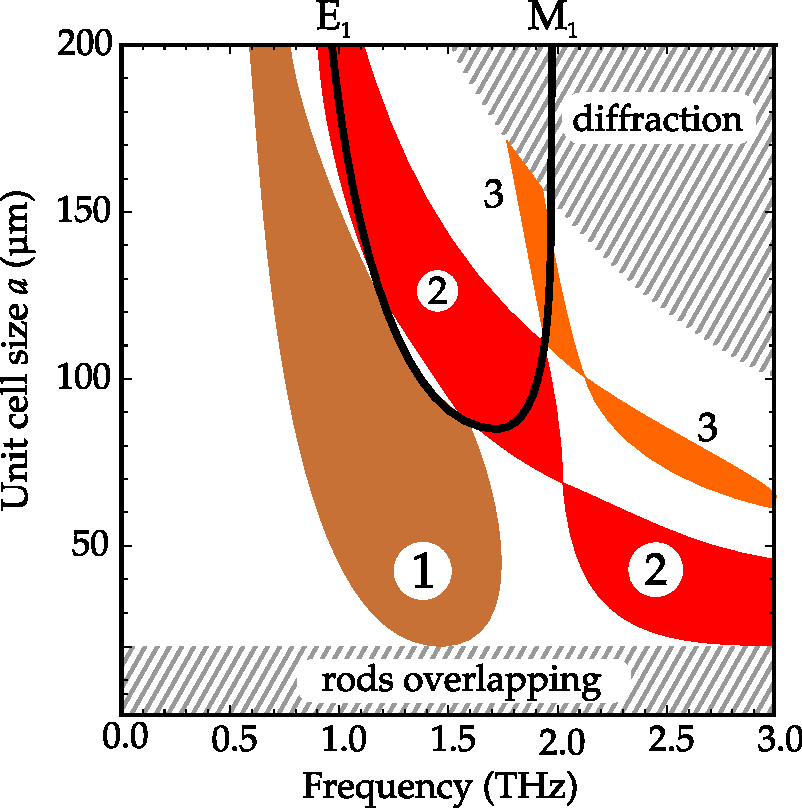
\includegraphics[width=7cm]{img/ERods_eps030_spacingscan_drawn_bands.pdf}
    \caption{Scheme of band gaps and Mie resonances for dielectric permittivity $\varepsilon_r = 30$. The Mie resonances shift to higher frequencies relative to the band gaps and no $\Neff'<0$ region is formed for any unit cell size (cf. Fig. \ref{fg_drawn100})}
\label{fg_drawn030}
\end{figure}

Note that the frequencies of the Mie resonances deviate from their free-space values when the rod distance is reduced. In fact, these resonances help to form the photonic band gaps (both Bragg and plasma band gaps) due to their dispersion. As a consequence, these resonances must be always located inside a frequency range with $\Neff''>0$.
%}}}
\paragraph{Discussion}%{{{
Having analyzed the case of high dielectric ($\varepsilon_r=100$) permittivity rods, we will draw below implications for building a negative-index MM from available dielectrics.  Another series of simulations implies that reducing the dielectric permittivity has the main effect to shift all the Mie resonances to higher frequencies (also with respect to the photonic bands). As a result, the band with $\Neff'<0$ gets gradually narrower and, for the rod permittivity below about 50, we do not find any cell size $a$ that would imply the first and second Mie resonances in the first photonic band as illustrated for $\varepsilon_r = 30$ in Fig. \ref{fg_drawn030}. This means that the value of $\varepsilon_{r} \approx 50$ is the minimum for obtaining a negative index of refraction in any square array of cylindrical rods. Note that one would come to a very similar value of minimum permittivity for the case of a square array of bars with a slightly different shape, e.g. a square cross-section. 

A sufficiently high permittivity can be found in the microwave and terahertz ranges, in a variety of materials, for example in titanium dioxide with $\varepsilon_r \approx 92$ \cite{nemec2009tunable} or in various ferroelectrics like strontium titanate \cite{skoromets2011tuning}. However, practical applications of the high-permittivity dielectrics in the THz range can be restricted by high dielectric losses due to low-frequency phonon absorption tails. To our knowledge, there is no material providing such a high permittivity in the near-infrared or optical ranges. This eliminates the possibility to build a MM at these frequencies with $\Neff'<0$ based on dielectric rods.

Finding a valid negative index of refraction $\Neff'$ for a photonic structure implies that the Snell law can be used to predict the negative refraction at an interface, provided the iso-frequency contours can be well approximated by a circle. This condition is fulfilled when the resulting wave vector is oriented close to a symmetry axis of the structure, or when the wave vector is negligible compared to the reciprocal lattice vector (i.e. $k\ll \frac{\pi}{a}$ and thus $|\Neff'| \ll \frac{c}{2af}$).  In the latter case the iso-frequency contours of the isotropic structure approach a circular shape near the $\Gamma$-point in the Brillouin zone center.  By contrast, the opposite implication is not necessarily applicable---a structure with a high enough spatial dispersion can still refract under negative angles, yet its refractive index computed along a symmetry axis never reaches negative values and the phase difference across each its unit cell is positive and can be comparable to $\pi$.  For example, it was suggested earlier  \cite{vynck2009all} that an array of silicon rods ($\varepsilon_r \approx 12$) can constitute a true left-handed metamaterial ($\Neff'<0$).  In agreement with the results presented above, we believe that the negative refraction is not a sufficient proof of $\Neff'<0$, which would require a much higher permittivity contrast than that of silicon.  We conclude that the electromagnetic behavior observed previously \cite{vynck2009all} has to be described by means of the PhC dispersion curves. 

We demonstrated that for $\Neff'<0$, not only the high permittivity contrast, but also a correct geometry is required. A wedge filled with an array of square-shaped high-dielectric bars was previously reported refracting under negative angles \cite{peng2007}. The high filling fraction ($0.44^{2}$) simultaneously with a permittivity of $\varepsilon_r \approx 600$ clearly qualified this structure as \textit{dense}. Using the above described approach, we computed its spectra qualitatively similar to Fig.~\ref{fg_spec}(c) and no band with $\Neff' < 0$ was resulting from our effective index retrieval. However, when we reproduced the wedge experiment numerically, our simulations confirmed that it does refract the light under negative angles.

This structure lies at the boundary between the criteria for MMs and PhCs described in the Introduction.  To determine its refraction angle, in general, it is not possible to use the concept of the effective refractive index and its iso-frequency contours have to be used instead (like in PhCs). At the same time, this structure was proved to partially retain negative refraction even under randomization of the positions of the dielectric bars \cite{peng2007}, implying that most of the resonant energy is concentrated inside the dielectric (which is characteristic of MMs).
%}}}



\begin{figure} \caption{img/ERods\_eps100\_R11\_PWEM.pdf}  \centering 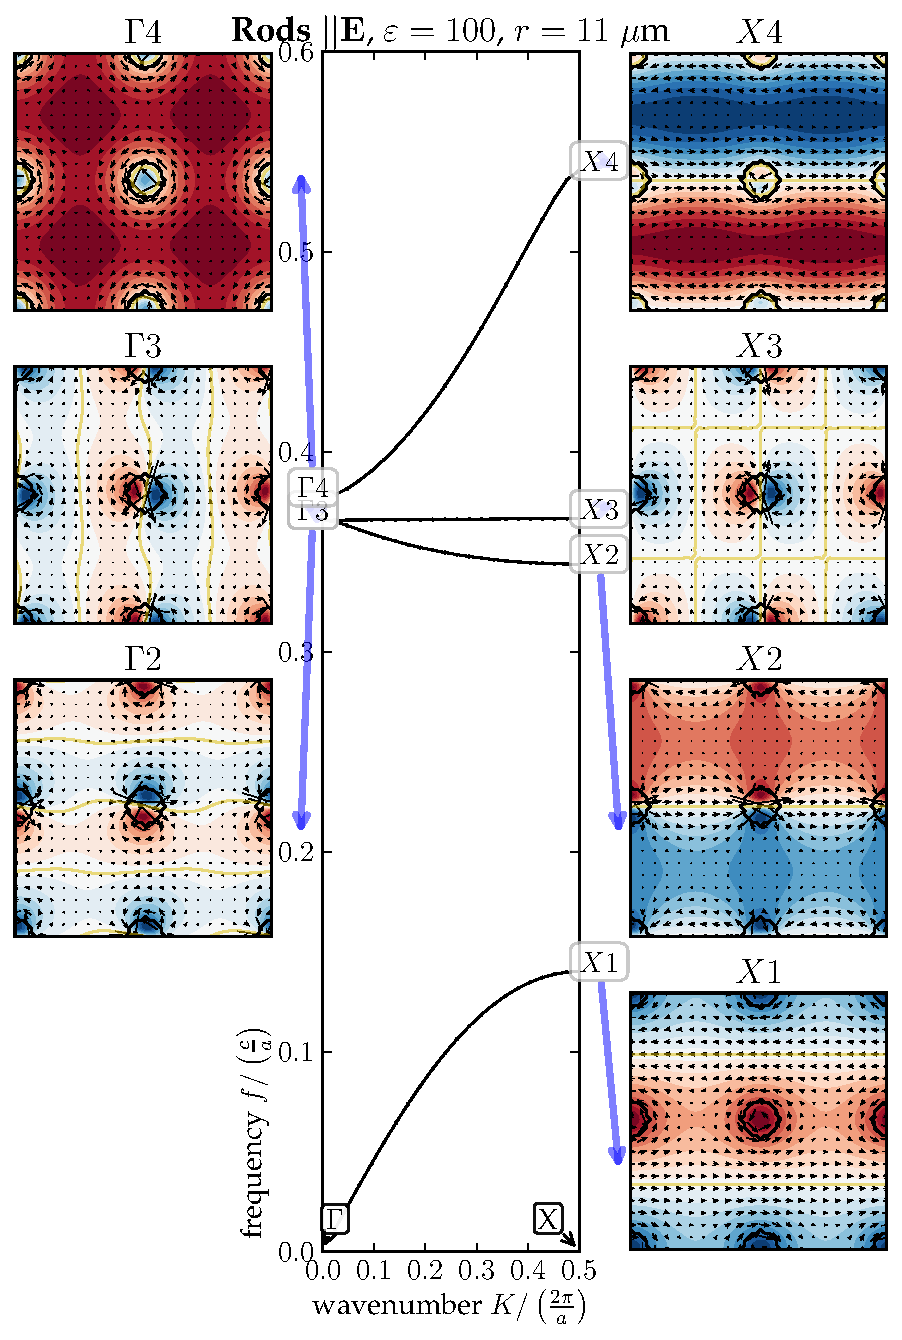
\includegraphics[width=10cm]{img/ERods_eps100_R11_PWEM.pdf} \end{figure} 
%  \begin{figure} \caption{img/ERods\_eps100\_single\_a120\_FDTD.pdf}  \centering 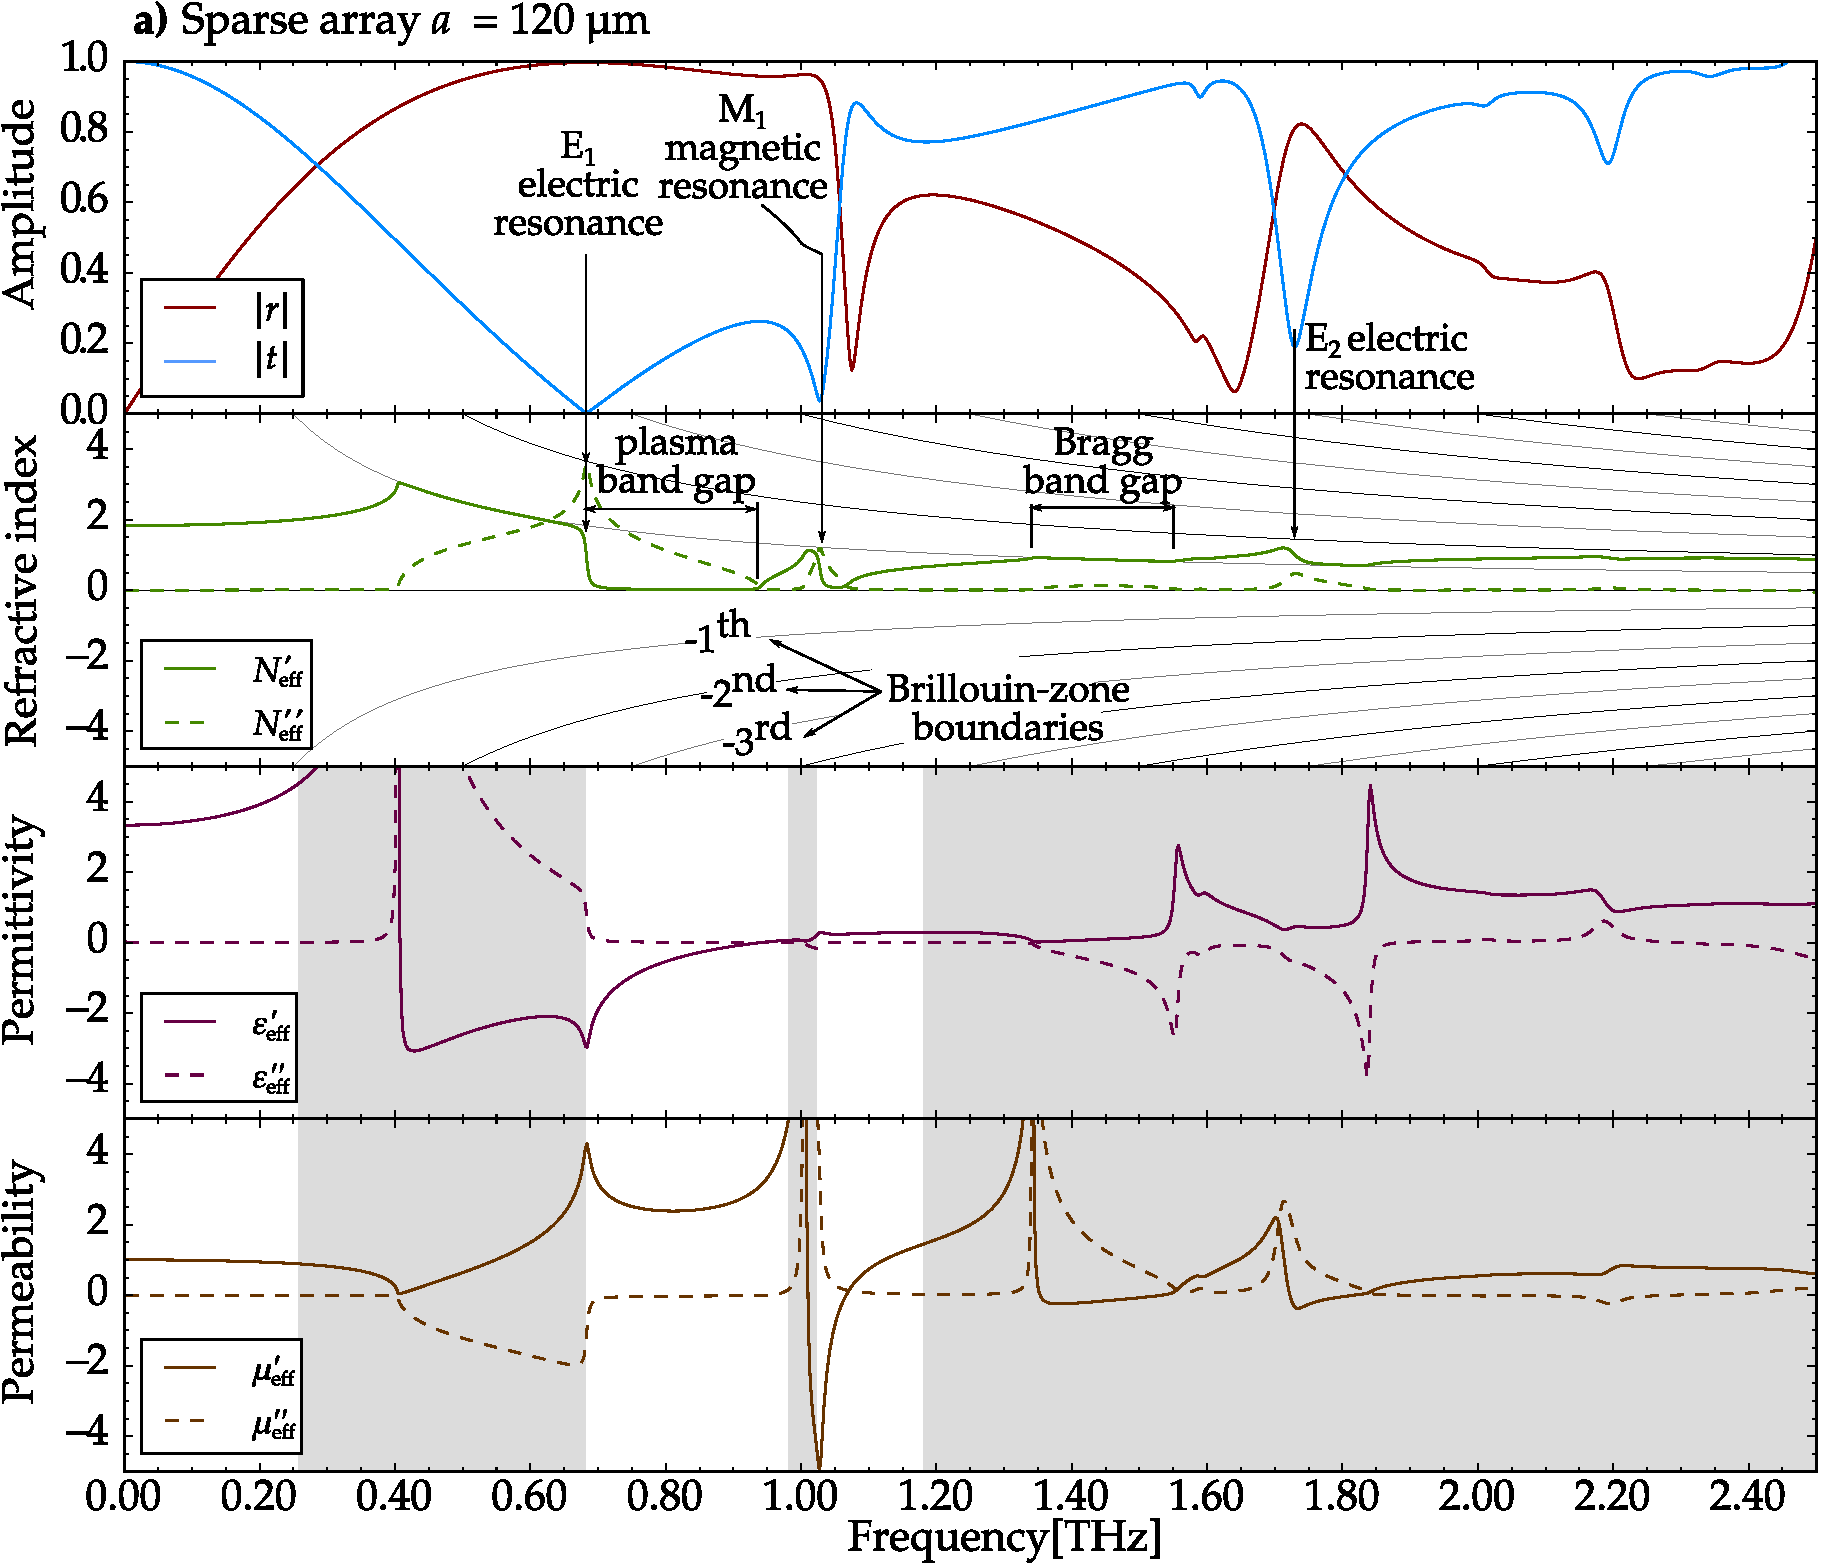
\includegraphics[width=10cm]{img/ERods_eps100_single_a120_FDTD.pdf} \end{figure} 
%  \begin{figure} \caption{img/ERods\_eps100\_triple\_a150a100a080\_FDTD.pdf}  \centering 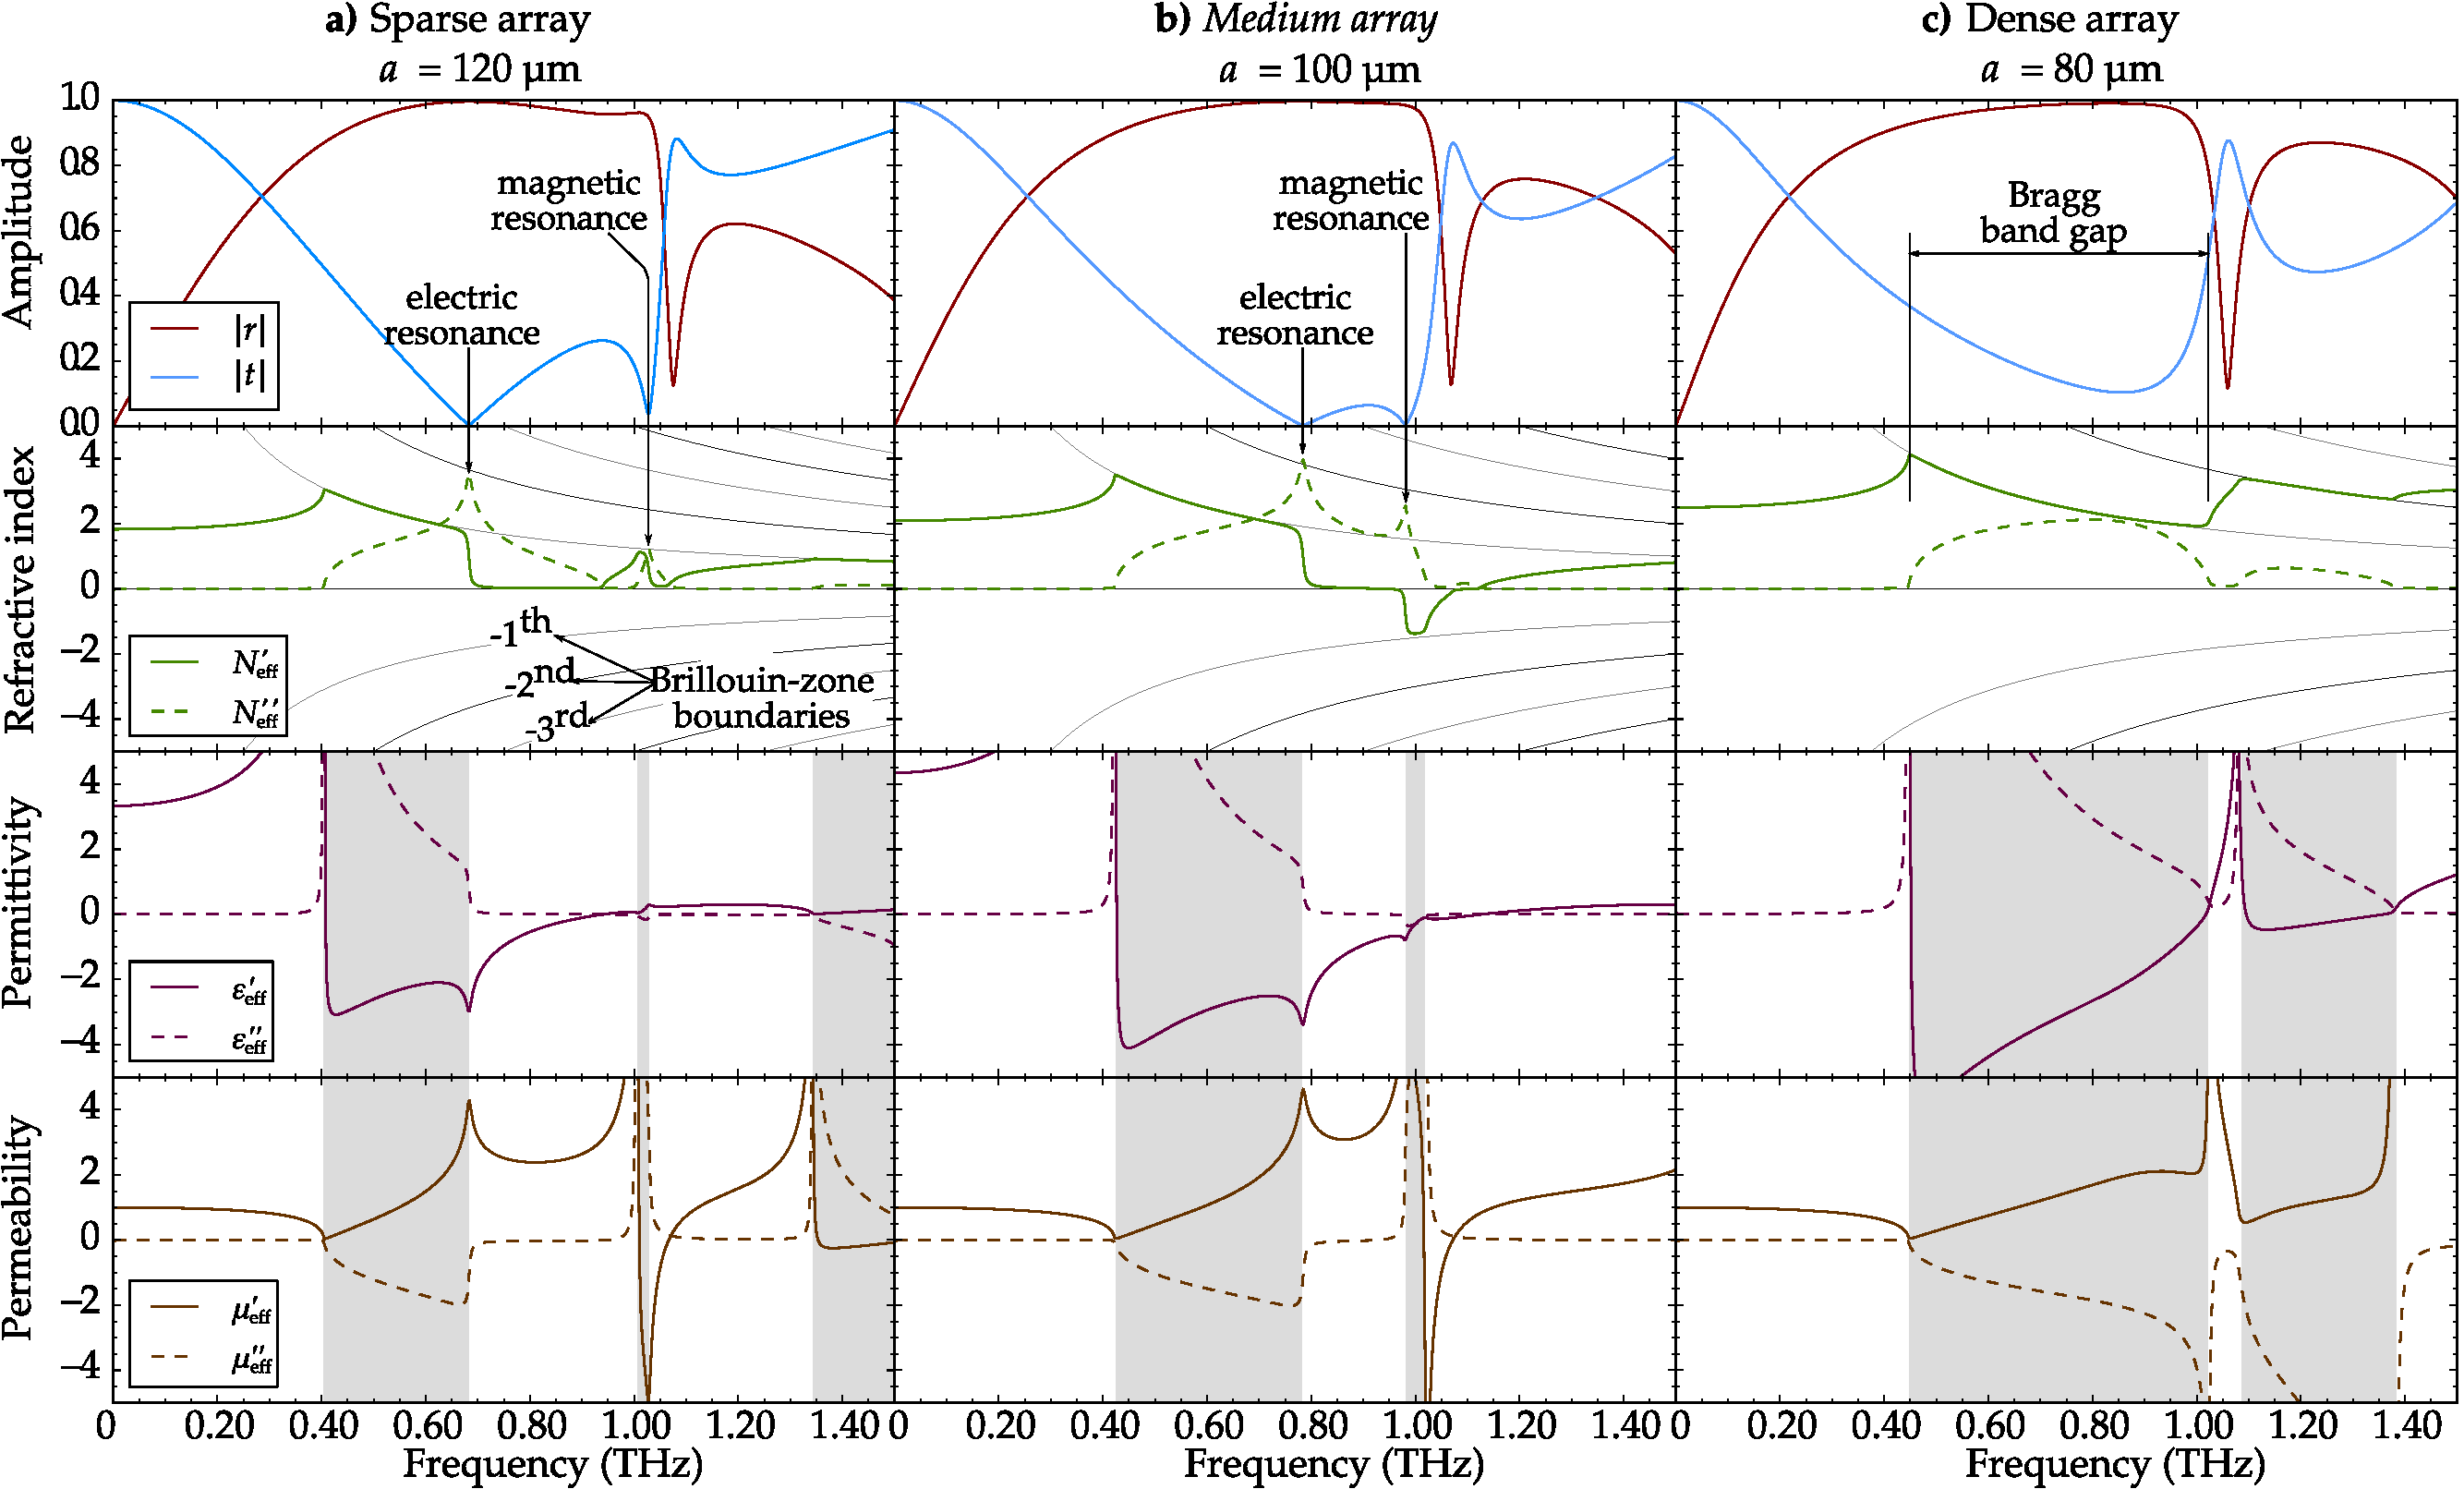
\includegraphics[width=10cm]{img/ERods_eps100_triple_a150a100a080_FDTD.pdf} \end{figure} 
%  \begin{figure} \caption{img/ERods\_forSeefeld\_sparserN\_denserN\_DrawnBands.pdf}  \centering 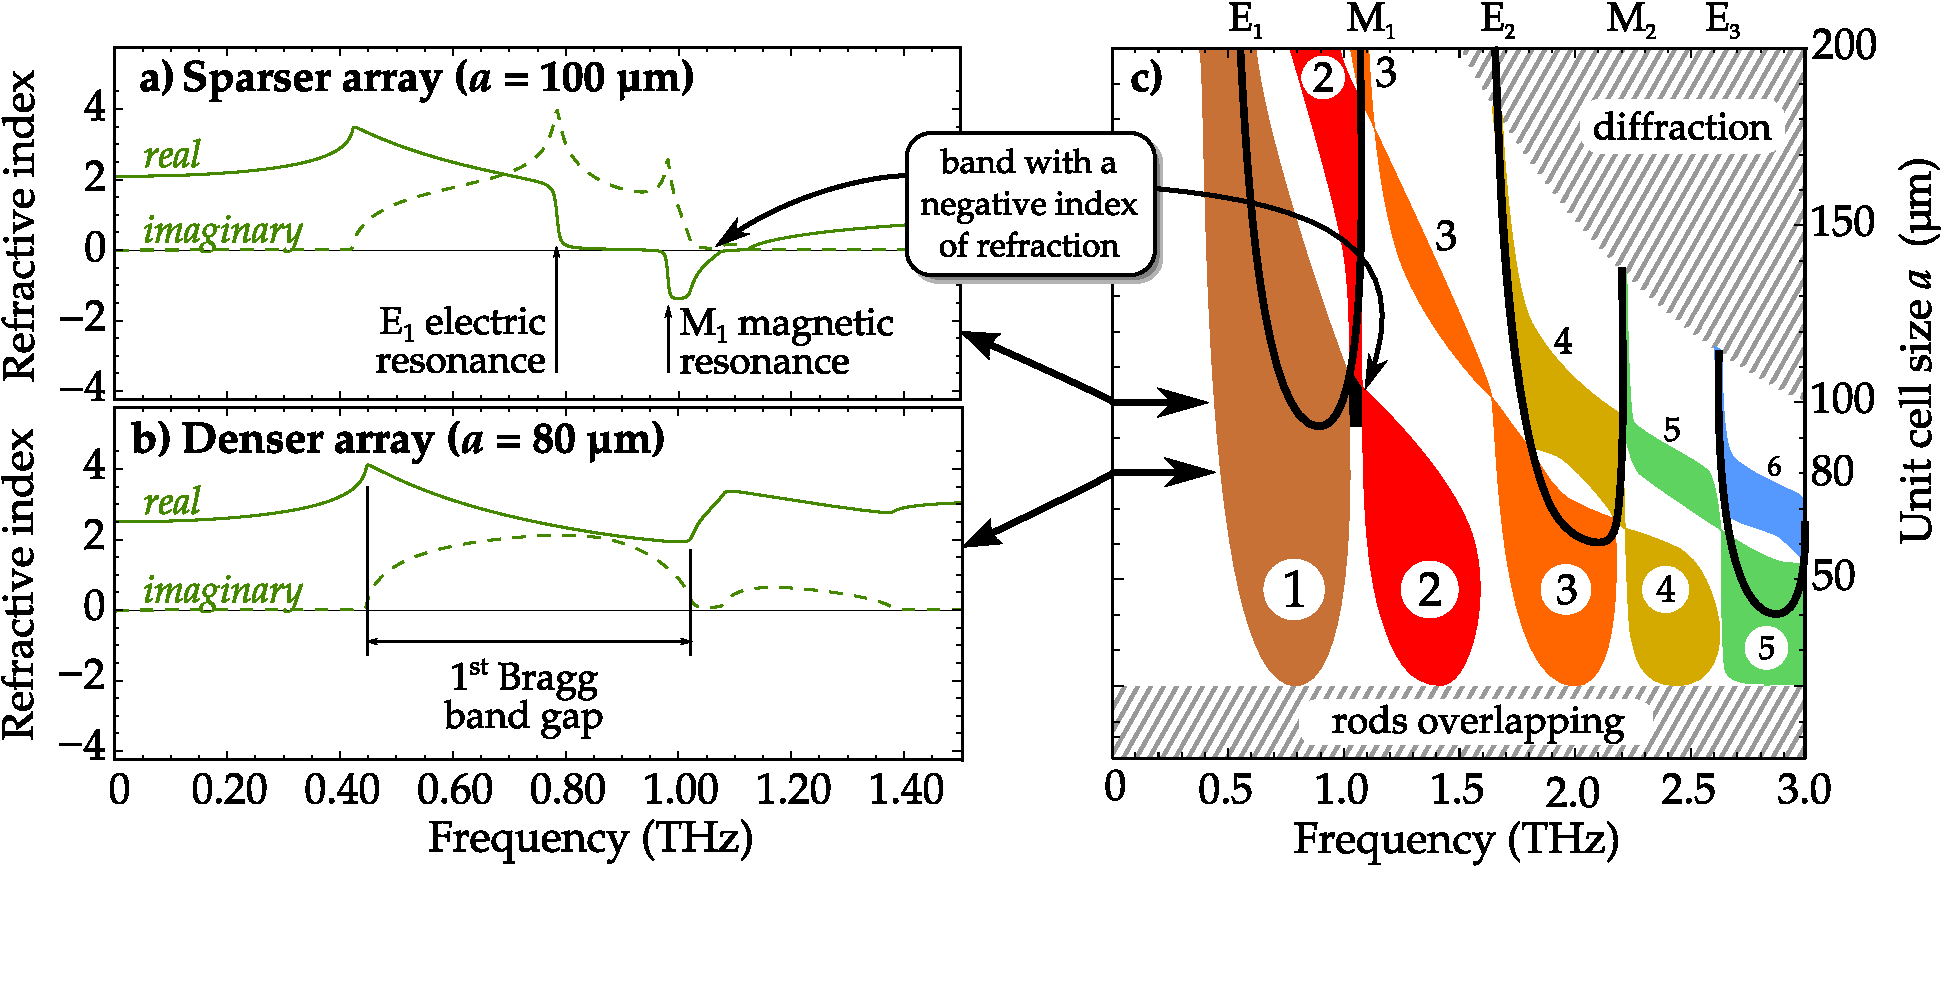
\includegraphics[width=10cm]{img/ERods_forSeefeld_sparserN_denserN_DrawnBands.pdf} \end{figure} 

\begin{figure} \caption{img/ERods\_sketch\_recordedline.pdf}  \centering  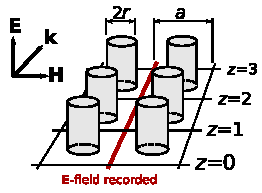
\includegraphics[width=10cm]{img/ERods_sketch_recordedline.pdf} \end{figure} 
\begin{figure} \caption{img/ERods\_eps100\_R10u5\_FXplot.pdf}  \centering 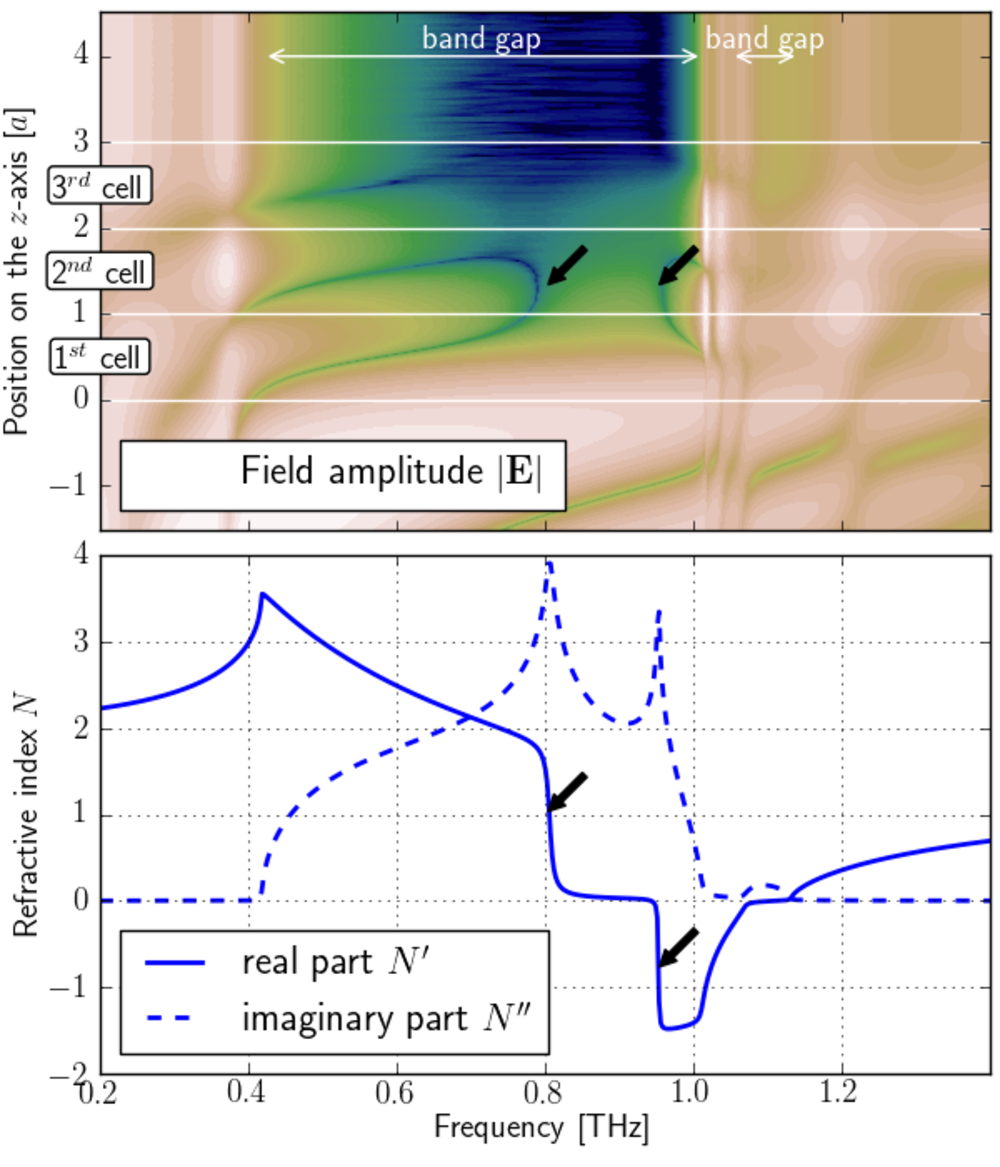
\includegraphics[width=10cm]{img/ERods_eps100_R10u5_FXplot.pdf} \end{figure} 







\FloatBarrier %====================================================================================================
\section{Metallic sheet with slits} \label{section_eot} % references to ->
Wood anomaly in hole arrays
Standing SPP wave






\FloatBarrier %====================================================================================================
\section{Fishnet -- metallic sheet with holes} \label{section_fishnet} % references to ->
%{{{
\paragraph{Extraordinary transmission}
\add{
	... EOT transmission --- Aperture-array transmission --- Wood anomaly --- standing surface plasmons

	... The resonance in the metallic mesh has been used as a filter \cite{ulrich1967effective,ulrich1967far}
	... has been known for half a century \cite{vogel1964transmission}

	... Improved cross-shaped pattern for better spectral selectivity \cite{porterfield1994resonant}
	}
\paragraph{Negative-index structures}


\add{
	Perforated plates \cite[p. 58]{brown1953artificial} % http://photonics.inescporto.pt/links/fct2013-1/metap14.pdf
	%Wood anomaly in slit arrays; 
	...  wave propagation can be also understood through the "hopping model"

	... fishnet achieves relatively low losses, since it is optimised for thick and short conduction paths 

	... asymmetric cladding of the sheet suppresses peak transmission, 
	surface plasmons, standing/propagating
	--> back reference to expe.tex:79

	%Babinet principle

	... appears hard to be homogenized by the s-parameters \cite{wang2010composite}

	% for nearly flat structures, where most of the fields are confined within a slab perpendicular to $\KK$, a

	\cite{yahiaoui2012metallo,rockstuhl2008light}
	}

\paragraph{Experimental results}
\add{
	... spectra of laser-drilled fishnets

	... Part of the fishnets were made of two foils as a metal-insulator-metal structure, but their spectra were also hard to interpret.

	... Our group received another fishnet sample made by automated mechanical drilling (Fig. \ref{fg_fishnet_mechanical}) into a double-sided circuit board blank, consisting of two 30 $\upmu$m copper foils glued to a plastic. The sample was measured by the terahertz spectroscopy yielding relatively complicated spectra, which could not be reasonably matched by any of the simulations. We assume that the clash between the measured and simulated values comes from the imprecision in the sample itself, namely from the burrs from drilling.
\begin{figure}[ht] \caption{A drilled fishnet with $500\times 500$ $\mu$m periodicity. The inclined view from the bottom side shows the burrs that were probably responsible for the large difference of the measured and simulated spectra.}  \centering 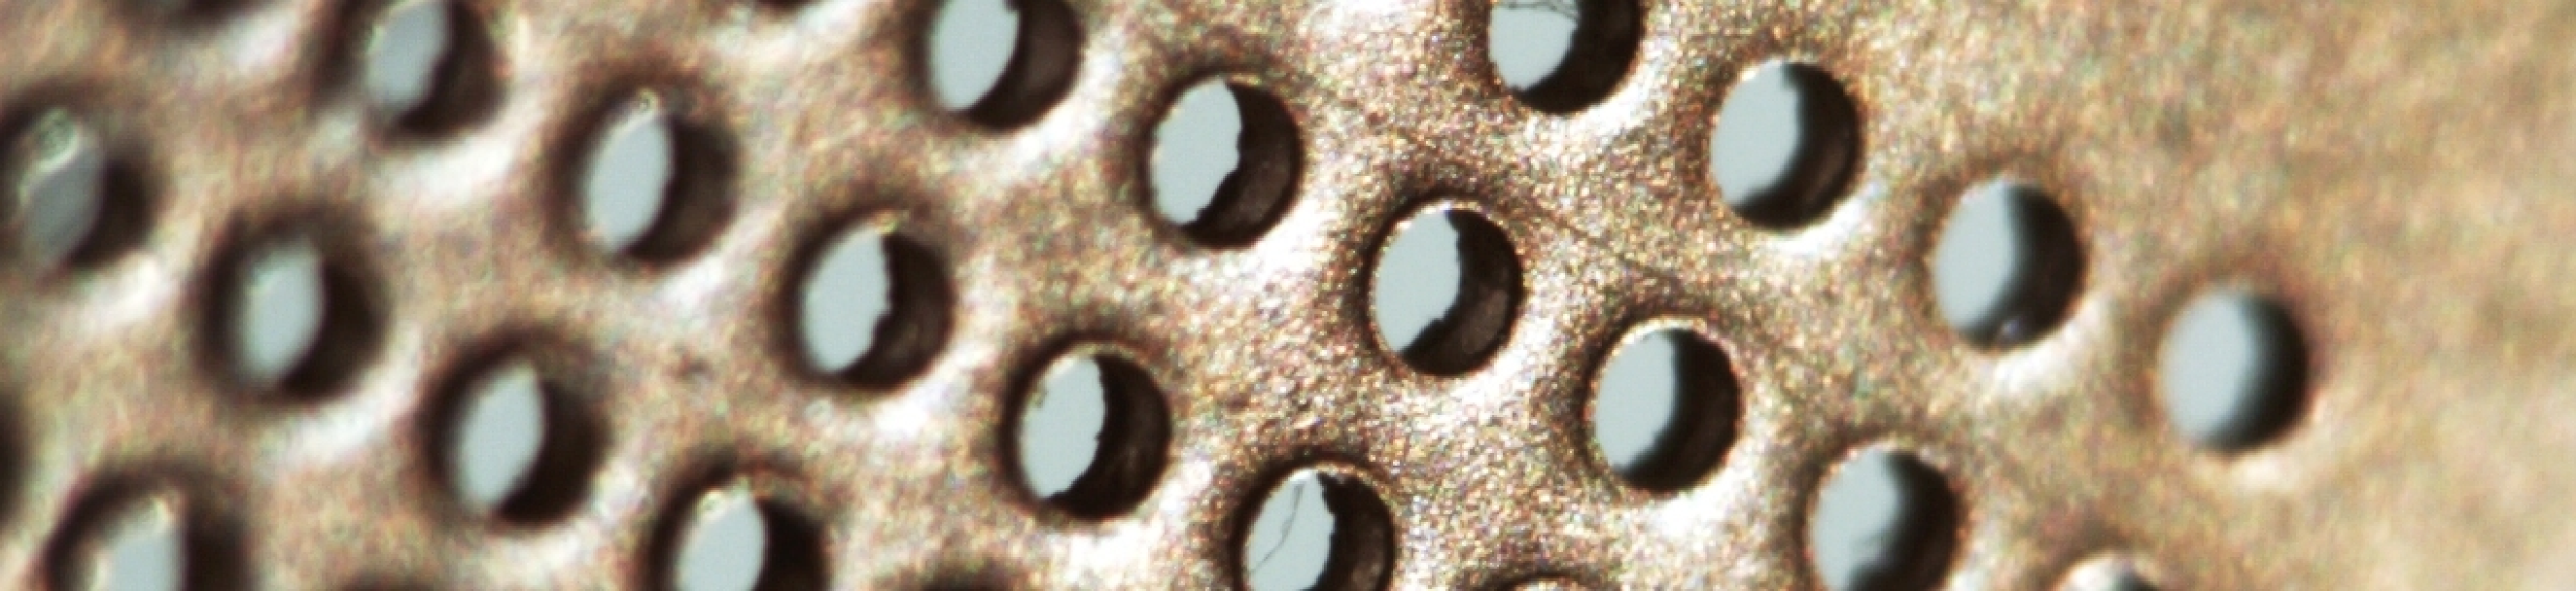
\includegraphics[width=.8\textwidth]{img/fishnet.pdf} \label{fg_fishnet_mechanical} \end{figure}
	}


%}}}


\FloatBarrier %====================================================================================================
\section{Other structures} % plasmonic spheres (note: resonance width determined by gamma of the metal?)
\cite{croenne2009controle}



%% TODO remaining topics to be added or checked: 
% 

%%	* PhCs with metallic/metamaterial inclusios, [Monsoriu, Lina Shi and friends]
	%thin wires [8], [28], Swiss rolls [9], SRRs [9], electric SRRs (eSRRs) [29], [30], pairs of rods [10], [12], [31], pair of crosses [32], fishnets [17], [33]”


